\section{Hardware Components and Construction}

\subsection{Light-Weight Mirror Prototype Construction}

The multifocal ellipsoidal mirror is the most critical component of the detector. A comprehensive R$\&$D program
was conducted for the purpose of addressing all of the key requirements and to find possible solutions, and to test
and verify the entire technological chain of building mirror prototypes on a 1:2 scale. All core parameters of the
detector were checked and/or derived from results of Monte Carlo (MC) simulations.

Because there is no mirror support structure, no additional material is introduced  within the acceptance, i.e. in
front of drift chambers. Therefore the major requirement we needed to satisfy was to build a light-weight and
self-supporting multifocal mirror consisting of many ellipsoidal mirror facets glued together along their edges. This
led to several problems to solve. One of them was to define contact surfaces of adjacent mirror facets that would
allow final assembly to be completed without any shape adjustments that left no gaps between them. An analytic
solution of a system of two second-order equations that describe two intersecting ellipsoidal surfaces leads to an
equation of fourth order in general form. The solutions for any two intersecting ellipsoidal mirrors of different
parameters have been used directly in the design: the line along which two ellipsoidal surfaces intersect is a flat
line of second order, i.e. that which entirely belongs to one particular well defined plane. This plane coincides with
the edge of each of two adjacent facets that had to be glued together.

One of the R$\&$D goals was to test this possible solution by building three scaled prototype ellipsoidal facets
forming a portion of the combined mirror. A complete set of tooling necessary for the thermal shaping of the
front and back films, manufacturing of the ellipsoidal substrates, assembly of the facets, and final trimming were
successfully designed, constructed, and tested. Some parts for tests are shown in Fig.~\ref{fig:Proto_4parts}.

\begin{figure}[ht]
    \centering
    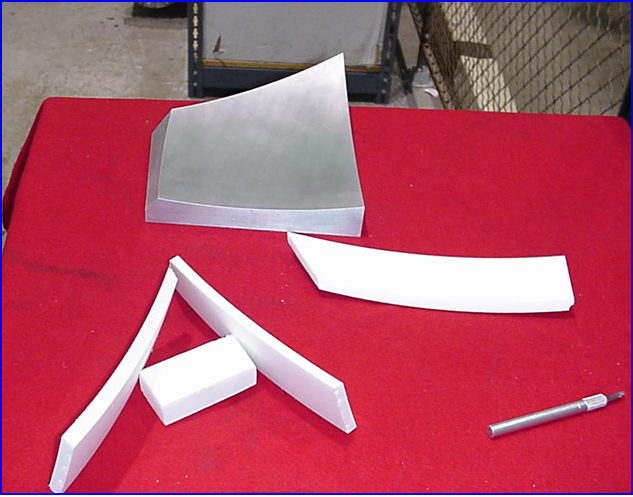
\includegraphics[width=1.0\linewidth]{images/Proto_4parts.png}
    \caption{Three prototype ellipsoidal foam mirror facets (bottom) and the spherical master table (top).}
    \label{fig:Proto_4parts}
\end{figure}

Three prototype facets (no reflective coatings on the substrates) were put together, touching each other exactly
as designed on the spherical working surface of the assembly table. The back of each facet was of the same
spherical shape. The facets were left under their own weight on the master table of the spherical working surface
for several months, (see Fig.~\ref{fig:Prototype}), to allow checking for any changes in shape and/or quality.

\begin{figure}[ht]
    \centering
    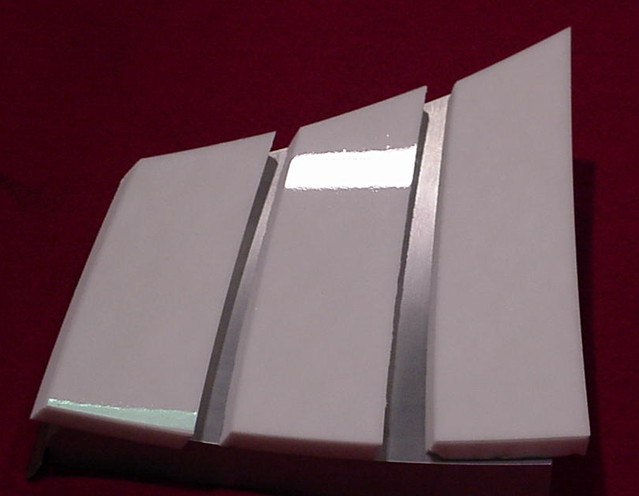
\includegraphics[width=1.0\linewidth]{images/Prototype.png}
    \caption{Three prototype ellipsoidal mirror facets on the spherical master table. They were placed so that they
      would not touch each other. This was in order to leave them free and to check their shape stability.}
    \label{fig:Prototype}
\end{figure}
We learned the following lessons:

\begin{itemize}
    \item Each substrate must have a multi-layer structure;
    \item The thickness of the substrate material had to be between 3/8~in and 3/4~in;
    \item The substrate material ROHACELL polymethacrylimide foam with a density up to 150~mg/cm$^2$ could be
      employed;
    \item The trimming technology had to be improved to provide increased precision of the mechanical processing and
      final assembly;
    \item In all gluing operations non-shrinking glues had to be used or a special technique had to be developed to avoid
      post-polymerization effects;
    \item Acrylic films of optical quality have to be used for the front and back surfaces of the mirrors;
    \item It is critical that there is structural stability of the mirror facets during the gluing process, which includes
      the complete polymerization time.
    \end{itemize}

The results obtained were useful in building the final multifocal mirror. Figure~\ref{fig:facet} shows one of the
ellipsoidal facets being prepared for the combined mirror assembly. Final assembly of a 1/12 portion of the full
mirror, consisting of five ellipsoidal coated mirror facets or one half-sector, is shown in Fig.~\ref{fig:Picture3}.

\begin{figure}[ht]
    \centering
    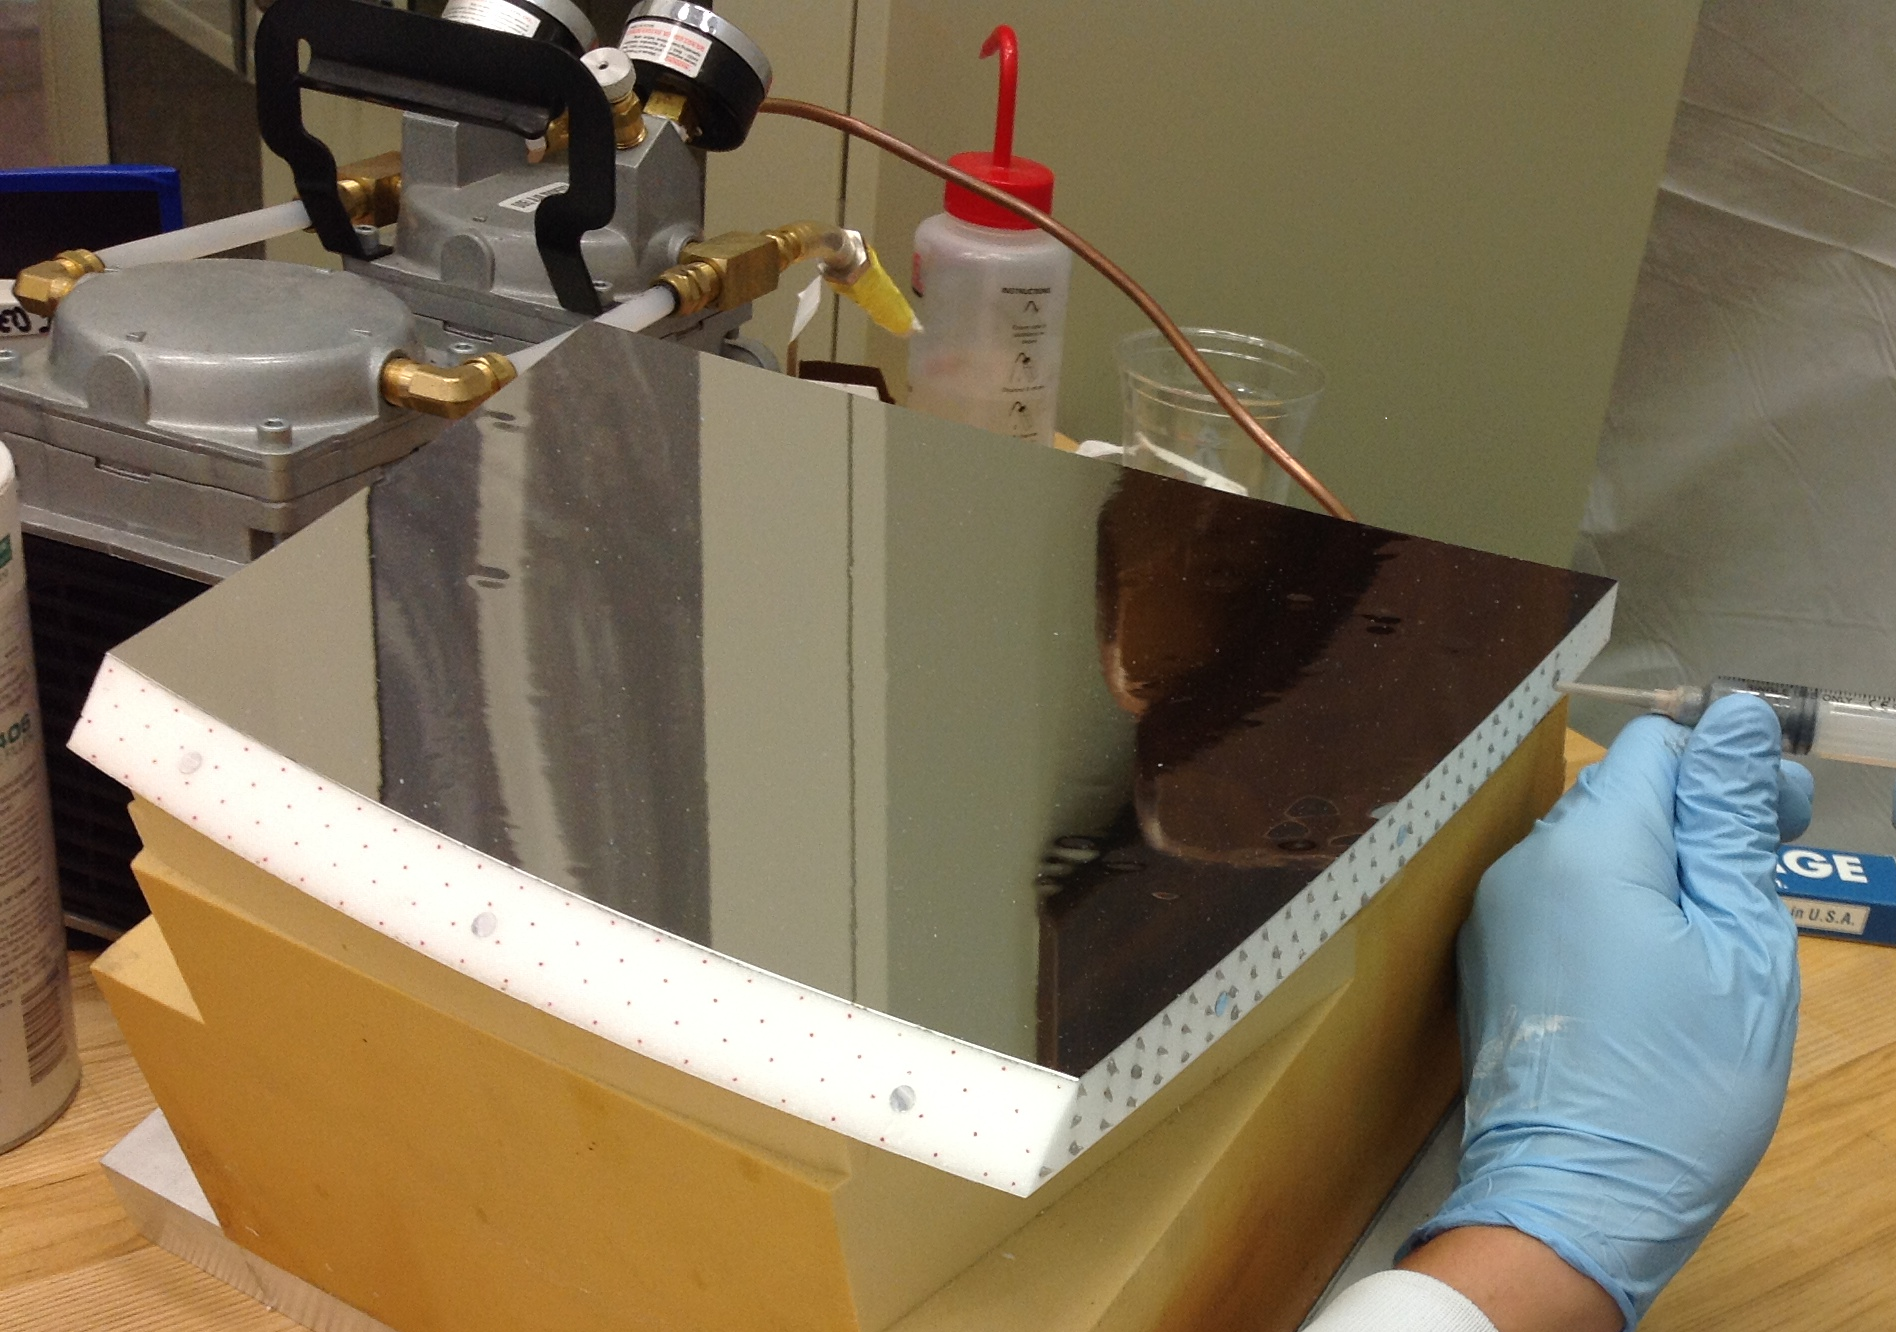
\includegraphics[width=1.0\linewidth]{images/Picture2.png}
    \caption{An ellipsoidal mirror facet with all four flat contact surfaces prepared for gluing.}
    \label{fig:facet}
\end{figure}
\begin{figure}[ht]
    \centering
    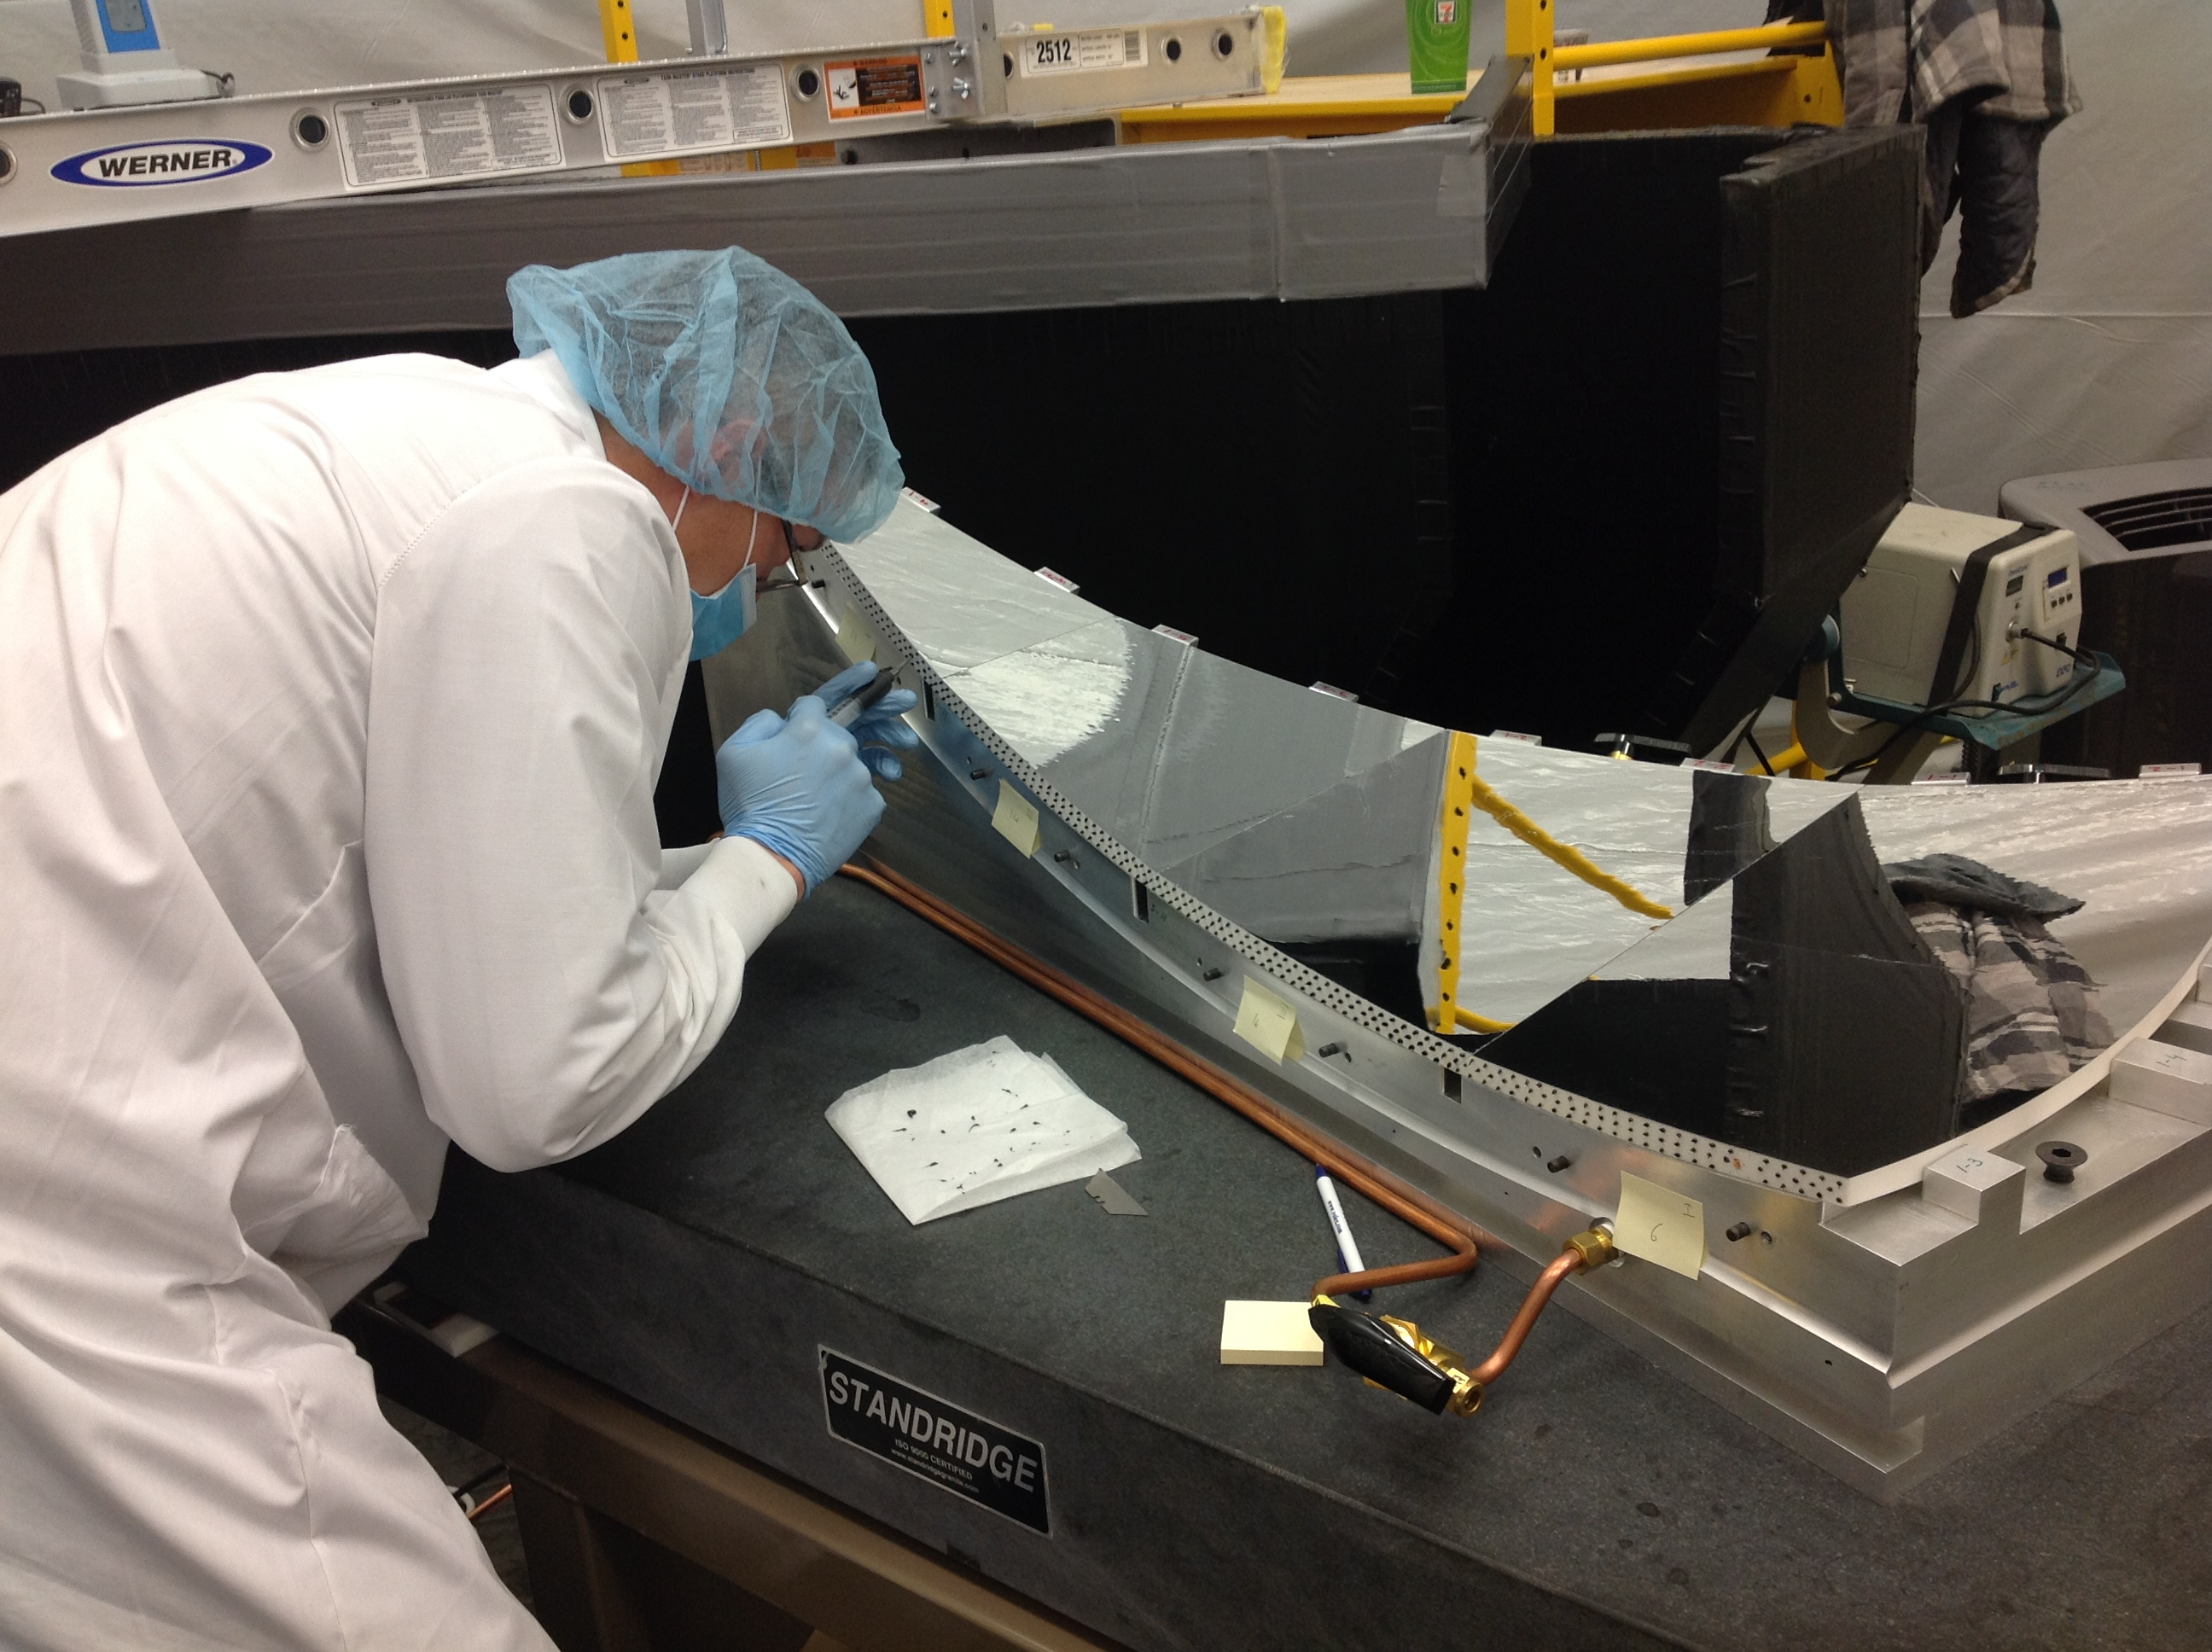
\includegraphics[trim={20cm 15cm 0 10cm },clip,width=\linewidth]{images/Picture3.JPG}
    \caption{Five ellipsoidal mirror facets glued together make up 1/12 of the full HTCC mirror (half of a CLAS12
      forward sector).}
    \label{fig:Picture3}
\end{figure}

\subsection {Ellipsoidal Mirror Facet Manufacturing}

The usage of high-accuracy mechanical processing was absolutely unavoidable in providing the high-precision mirror
facets for the final combined mirror. Putting together 60 ellipsoidal facets of semi-trapezoidal shape, fitting against
each other without adjustment of the overall dimensions of the adjacent facets seams, is a difficult task. In order to
adjust the facets of the combined mirror, each individual facet would need to have its own support infrastructure,
and this would unavoidably introduce additional material. With these concerns in mind, all of the mechanical processing
of the mirror facets was performed with a HAAS 5-axis milling machine. This allowed us to develop and use special
trimming technology for the facets. One such technique was the ``one shot" method, which provided the ability from
one setting to trim any facet with 3 or 4 contact surfaces that needed to be glued. This was done to exclude, or at
least minimize, the errors introduced when we reset the orientation of the facets while we cut 3 or 4 edge planes
under different combinations of angles. We estimated that any deviation in the designed dimensions of more than
about 0.005~in would make the combined, precision assembly of so many mirror substrates impossible. This was
because any post-manufacturing adjustment of any of mirror substrates was not an option. In no way could two facets
be found to be either overlapping or with significant gaps between them. These gaps could be as wide as the thickness
of a regular glue joint obtained by simple contact pressure. Otherwise, if these gaps were any larger, they would
reduce the working acceptance and lead to reduced detector efficiency.

The polishing process of large mirrors (8-9~ft diameter) usually means that the manufacturing process is both
labor intensive and time consuming, thus leading it to be very expensive. Therefore, we looked for solutions to
completely avoid any polishing. Due to the fact that we did not require sharp images, the mirror facets were thus
constructed to only work as efficient light collectors. To accomplish the goal we developed and established an entire
assembly procedure, followed by tests of the construction and rating of the final results.

Another issue we addressed was the choice between gluing or mechanical plug-pin assembly procedures. Clearly
gluing introduces deformations due to the shrinkage of any glue. On the other hand, an assembly procedure that
uses location pins results in a more complicated joint since it requires the high-precision processing of plastic foam
parts that are both very light-weight and mechanically weak. Moreover, if any joint deformation was observed after
the first assembly attempt, then many of the parts involved (including the mirror facets) could not be
re-manufactured or used again.

We built 12 identical half-sectors of the combined mirror. Each half-sector consists of 4 ellipsoidal mirrors of
different parameters. The outermost mirror was too large to trim due to the limited travel of the milling machine
table. Therefore, this particular mirror was made of two substrates that were a mirror image of each other.
Consequently each half-sector includes 5 mirror substrates and the full HTCC mirror consists of 60 ellipsoidal
mirror facets in total. 

All mirror facets have the same composite (sandwich) structure: acrylic film (thickness 0.010~in) + foam (thickness
0.600~in) + acrylic film (thickness 0.010~in). The mirror substrate was made from ROHACELL PMI
(polymethacrylimide) foam and the acrylic films were of optical quality. Manufacturing any substrate was a
multi-stage process:
\begin{itemize}
    \item Thermal shaping of the acrylic film shells for the front (ellipsoidal) and back (spherical) of the mirror;
    \item Manufacturing of the foam substrates;
    \item Assembly (gluing) of the sandwiched mirror substrate;
    \item Trimming of the sandwiched mirror substrate;
    \item Coating of the ellipsoidal faces of the substrate;
    \item Reflectivity tests of the mirror substrate.
    \end{itemize}

Correspondingly we used 5 different sets of high-precision, custom-made tooling for the thermal shaping, gluing,
and trimming of the substrates. The thermal shaping was done in a low temperature Precision oven with better than
0.5$^\circ$C  temperature uniformity in the volume. The tooling set for the manufacturing of mirror facet \#2,
which covers the polar angle in range $\theta = 12.5^\circ - 20^\circ$ and the azimuthal angular interval of
$\Delta \phi = 30^\circ$, is shown in Fig.~\ref{fig:Tool_on_tbl}.

\begin{figure}[ht]
    \centering
    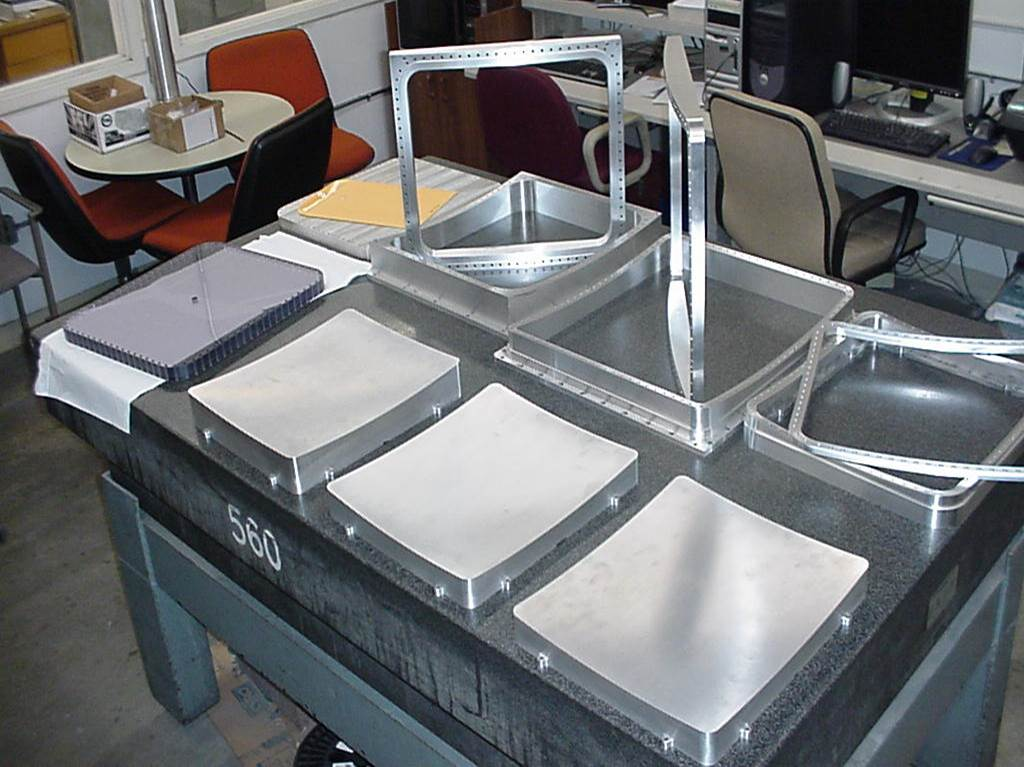
\includegraphics[width=1.0\linewidth]{images/Tool_on_tbl.jpg}
    \caption{Tooling set for the manufacture of mirror facet \#2.}
    \label{fig:Tool_on_tbl}
\end{figure}

The scheme of shaping the acrylic shells is illustrated in  Fig.~\ref{fig:Shaping_new}. Figure~\ref{fig:Vac_Mol_Back}
shows the partially loaded tooling set for shaping the back shell of the mirror in the oven. The shaping process was
done at temperatures of about 105$^\circ$C and differential pressures below 1~atm. There were two possibilities to
shape the shells: use vacuum shaping or just pressurizing the volume up to 2-3~psi differential. Since the tooling parts
were heavy and therefore required a relatively long time to reach the required temperature, the operations with the
oven would take about 3-4~hours, and the whole process of shaping one shell (load the tooling, heat it up in the oven,
cool down to room temperature, and unload the tooling) would take up to 5 hours.

\begin{figure}[ht]
    \centering
    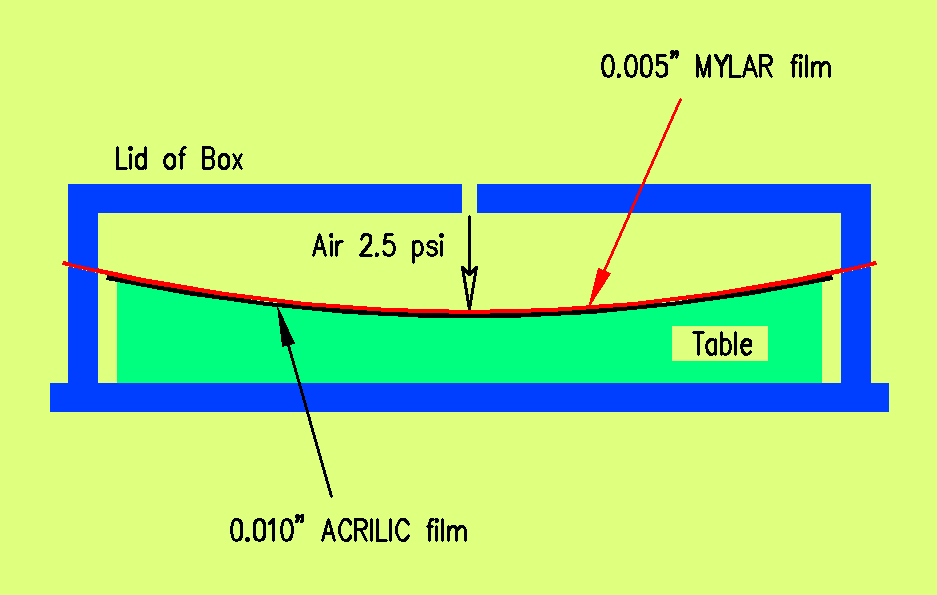
\includegraphics[width=1.0\linewidth]{images/Shaping_new.png}
    \caption{Scheme of thermal shaping of the spherical shell for the back of the mirrors.}
    \label{fig:Shaping_new}
\end{figure}

The loaded tooling set for shaping the front ellipsoidal shell in the oven by pressurizing the volume above the film is
shown in  Fig.~\ref{fig:Pres_Shaping_Front}. Figure~\ref{fig:Shell} shows the shaped acrylic shell for the front of
the mirror.

\begin{figure}[ht]
    \centering
    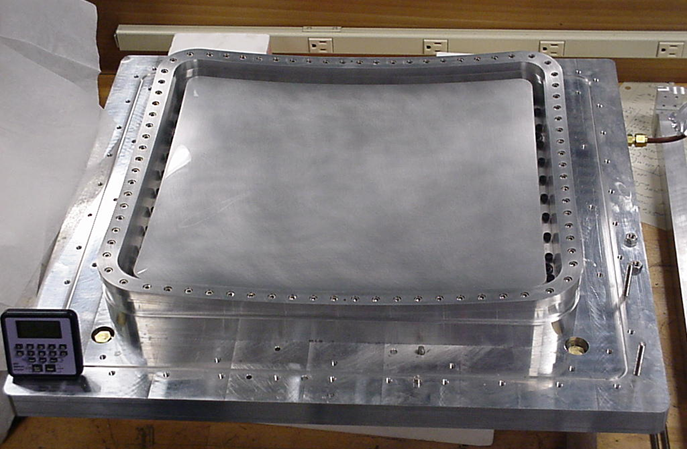
\includegraphics[width=0.95\linewidth]{images/Vac_Mol_Back.png}
    \caption{Partially loaded tooling set for shaping the spherical back shell of mirror facet \#2.}
    \label{fig:Vac_Mol_Back}
\end{figure}

\begin{figure}[ht]
    \centering
    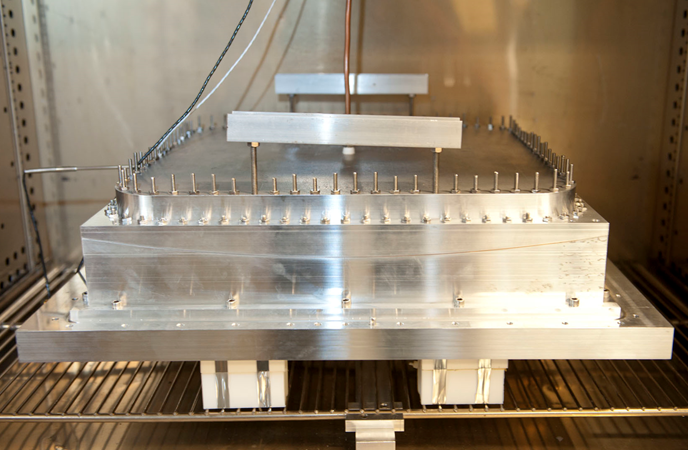
\includegraphics[width=0.95\linewidth]{images/Pres_Shaping_Front.png}
    \caption{Loaded tooling set for shaping the front ellipsoidal shell of mirror facet \#2 in the oven by pressurizing
      the volume with dry air using 1/4~in copper tubing.}
    \label{fig:Pres_Shaping_Front}
\end{figure}

\begin{figure}[ht]
    \centering
    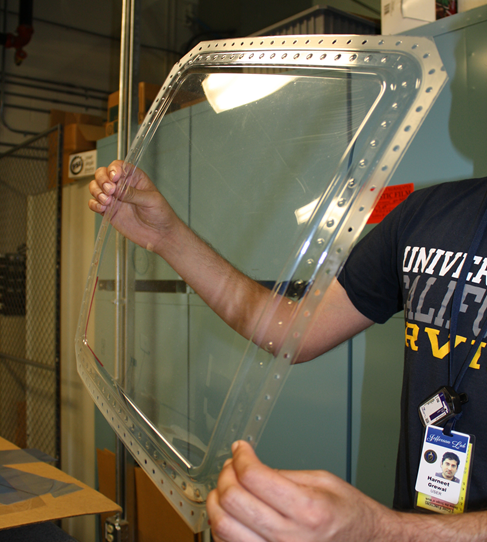
\includegraphics[width=0.90\linewidth]{images/Front_Shell.png}
    \caption{Thermally shaped front ellipsoidal shell for mirror facet \#2.}
    \label{fig:Shell}
\end{figure}

The cut-out of the foam substrate and processing of the back surface of spherical shape was performed without
using any custom-made tools, see Fig.~\ref{fig:Cut_Substr}.
\begin{figure}[ht]
    \centering
    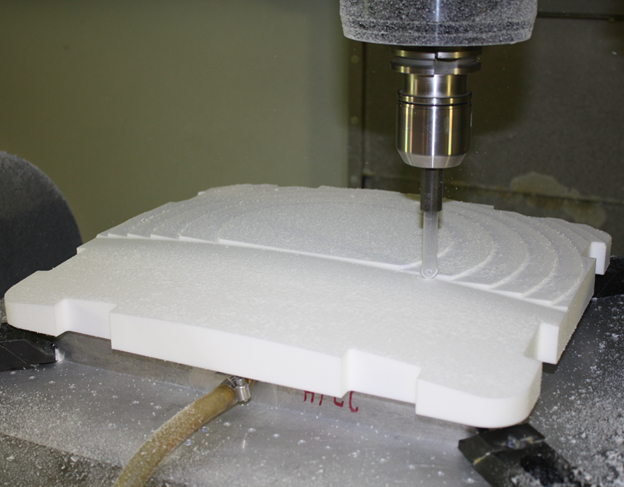
\includegraphics[width=0.9\linewidth]{images/Cut_Substr.png}
    \caption{Milling the back surface of the foam substrate for mirror facet \#2.}
    \label{fig:Cut_Substr}
\end{figure}

The front ellipsoidal surface was cut using the tooling that was also used for the final trimming of the sandwiched
glued facet. Once the front surface was cut, the facet was taken off the tooling set for the next operation of
gluing the acryl-foam-acryl sandwich. Figure~\ref{fig:Foam_Sub} shows the fully processed foam substrate for
mirror facet \#2 ready for the assembly of the sandwich. The scheme for the assembly of the sandwiched substrate
is shown in Fig.~\ref{fig:Gluing_Sandwich}. In Fig.~\ref{fig:Assembled_Sandwich} the fully assembled sandwiched
substrate for mirror facet \#2 ready for the final trimming is shown. 

\begin{figure}[ht]
    \centering
    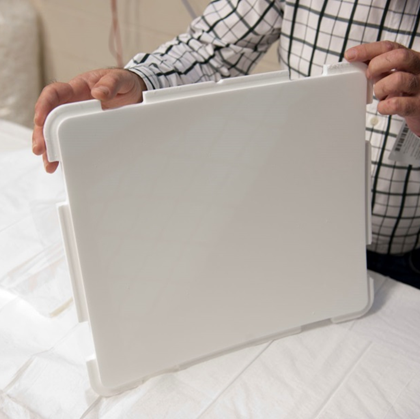
\includegraphics[width=0.9\linewidth]{images/Foam_Sub.png}
    \caption{A completed foam substrate that forms the core of the mirror facet.}
    \label{fig:Foam_Sub}
\end{figure}

\begin{figure}[ht]
    \centering
    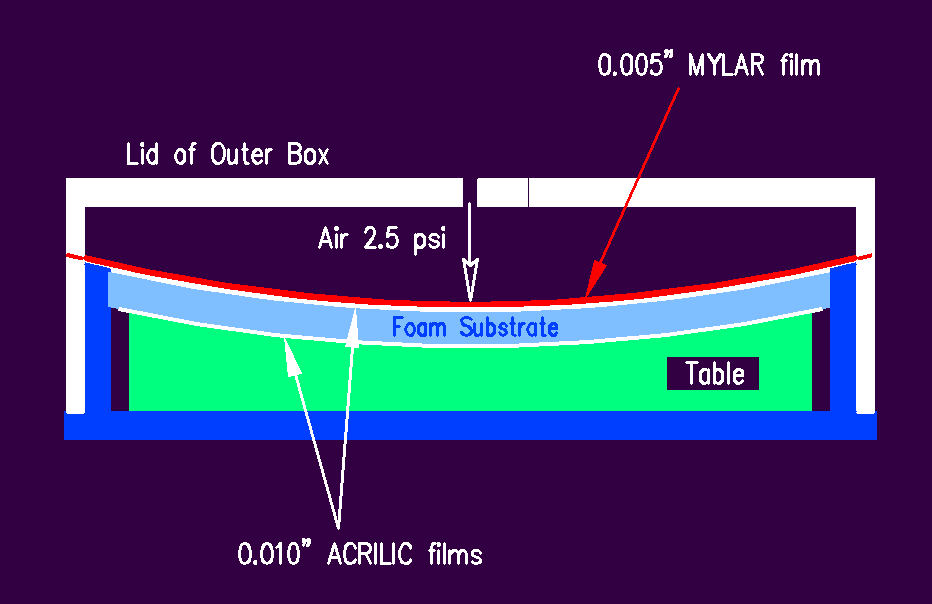
\includegraphics[width=0.9\linewidth]{images/Gluing_Sandwich_New.png}
    \caption{Scheme for gluing of the sandwiched mirror substrate.}
    \label{fig:Gluing_Sandwich}
\end{figure}
 
\begin{figure}[ht]
    \centering
    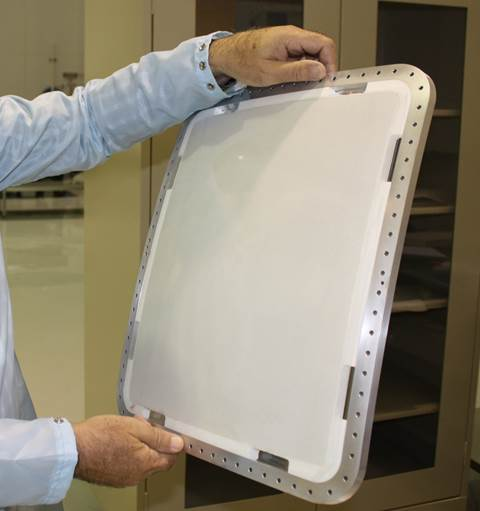
\includegraphics[width=0.9\linewidth]{images/Assembled_Sandwich.jpg}
    \caption{Sandwiched mirror facet after gluing components as shown in Fig.~\ref{fig:Gluing_Sandwich}.}
    \label{fig:Assembled_Sandwich}
\end{figure}

After gluing of the sandwich, it was put back in the tooling set for the final precision trimming. The shells were
designed and processed in a way that allowed  unequivocal and simple alignment of all parts during assembly. Using
the same set of tooling for cutting the face and trimming the facet, guaranteed automatic perfect relative
alignment of the parts being glued together. The accuracy of alignment, see Fig.~\ref{fig:Assembled_Sandwich},
and, therefore, the reproducibility of the results was achieved. Before the trimming operation, the front working
face of the substrate was covered with a special tight-fitting protective film to prevent damage or pollution of the
working surface while trimming the substrate. For better control of the uniformity of glue application (thickness,
formation of unwanted bubbles), the first manufactured mirror facet was assembled using epoxy glue with black
dye. The trimming was done in two steps. In order to avoid the front shell peeling off the foam, the substrate  was
cut through the front shell only using very small diameter (0.006~u=in) end mill, see Fig.~\ref{fig:Trimming_1}. Then
the outer portion of the shell was safely peeled off the substrate and the remaining trimming was performed using
a long end mill. The completed final trimming of the facet is show in Fig.~\ref{fig:Trimming_2}.

\begin{figure}[ht]
    \centering
    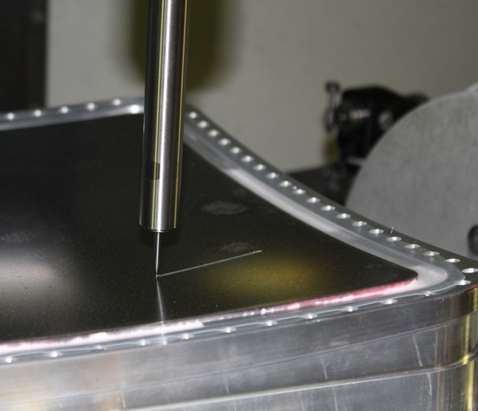
\includegraphics[width=1.0\linewidth]{images/Trimming_1}
    \caption{Cutting through the acrylic shell of the substrate using a small diameter end mill.}
    \label{fig:Trimming_1}
\end{figure}

\begin{figure}[ht]
    \centering
    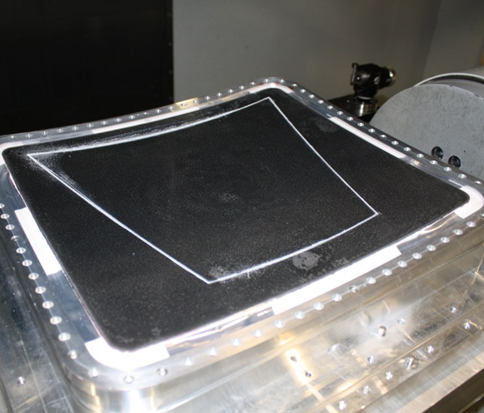
\includegraphics[width=1.0\linewidth]{images/Trimming_2}
    \caption{Completed final trimming of mirror facet \#2.}
    \label{fig:Trimming_2}
\end{figure}

During final milling the substrate was secured in place by inserting soft foam wedges along the partially cut sides
and glued to the outer portion of the substrate being trimmed. This completely eliminated any vibration that could
ruin the accuracy of the processing. Figure~\ref{fig:Trimmed} shows the completed mirror facet \#2 ready for
deposition of the reflective coating. All substrate trimming was done without any re-positioning of the facet during
the procedure. 

\begin{figure}[ht]
    \centering
    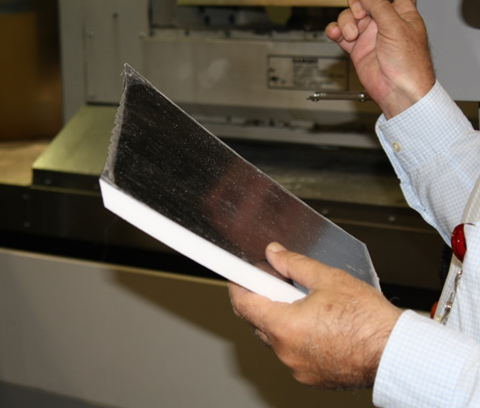
\includegraphics[width=1.0\linewidth]{images/Trimmed}
    \caption{Completely trimmed mirror facet \#2 covered with protection film. }
    \label{fig:Trimmed}
\end{figure}

The face of the mirror substrate did not require any processing before deposition of the reflector material. The
total thickness of the mirror is 130-135~mg/cm$^2$. Acrylic films were glued to both sides of the substrates to
compensate deformation introduced by the shrinking of the thin epoxy glue layers. No shrinkage effects in any of
the produced substrates was observed, thus long-term problems with mirror shape were completely eliminated.
All critical mirror fabrication steps were performed in a clean room (Class 1000). In addition, for better results,
all parts were individually cleaned using an ionizing gun right before assembly. As well, the clean room included a
clean bench with a HEPA air filter next to the assembly table that blowed filtered air over the table. Thermal and
mechanical processing was done either with protection films covering critical surfaces or encapsulated in a gas-tight
volume to prevent dust or any other unwanted depositions from damaging the working surface or otherwise
compromising the mirror reflectance.

\subsection{Tests of Mirrors Coated with Reflective Material}

Evaporated Coatings Incorporated (ECI) was chosen from among four potential vendor companies to perform
vacuum deposition of the reflective coating onto the HTCC mirror substrates.Test samples (flat sheets of acryl,
one untouched and one subjected to the same thermal shaping process used to form the front and back surfaces of
the mirrors) coated by ECI were the most reflective over the entire wavelength range of interest. A 30~W
deuterium lamp was used as a UV source from 200-400~nm, and a 50~W quartz-tungsten halogen (QTH) lamp was
used as a source of visible light from 370-650~nm. A monochromatic test beam for the reflectivity measurements
was generated by a Newport model 74125 computer-controlled monochromator. A Newport model 10Z40Al.2 flat
broadband mirror was used as a repeatable reference standard for the reflectance measurements. The mirror
consists of a UV-enhanced aluminum coating on a 1/4-in thick, 1-in diameter Zerodur substrate, with a protective
overcoat of UV-transparent magnesium fluoride to prevent oxidation. The custom coating material used by ECI has
an acceptable reflection coefficient in the UV-range and is resistant to oxidation at room temperatures. Each mirror
facet was coated individually and then tested at the company. The final quality control measurements of the coated
mirror facets was done at Jefferson Lab. Figure~\ref{fig:JLab_Mirror_Better} shows typical results of the
reflectance  measurements of an ellipsoidal mirror facet for the HTCC. The measured reflectance of the mirror
facet (black dots) is very close to the specification shown by the dashed curve. The reflectance of the reference
flat 1-in diameter mirror specified by the vendor and checked at Jefferson Lab is shown in Fig.~\ref{fig:Ref_Mirror}.
The measurement technique has small systematic uncertainties of about 1-2\%.

\begin{figure}[ht]
    \centering
    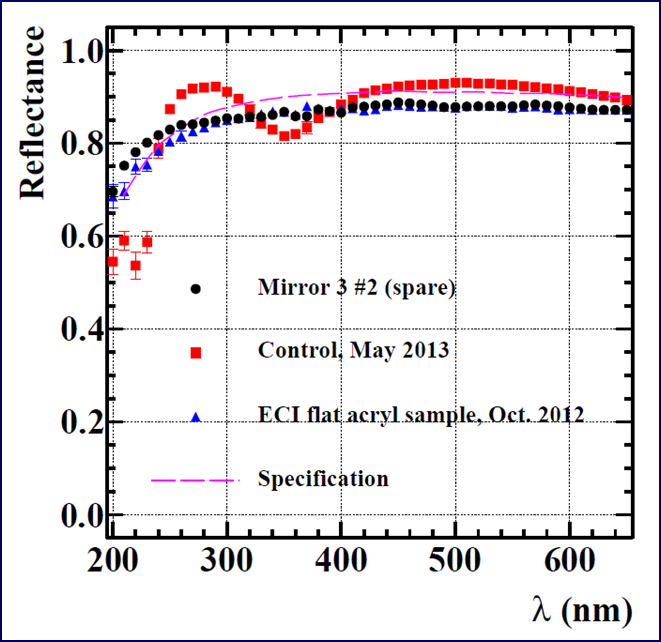
\includegraphics[width=1.0\linewidth]{images/JLab_Mirror_Better.png}
    \caption{Typical reflectivity of an ellipsoidal HTCC mirror facet as measured at JLab.}
    \label{fig:JLab_Mirror_Better}
\end{figure}

\begin{figure}[ht]
    \centering
    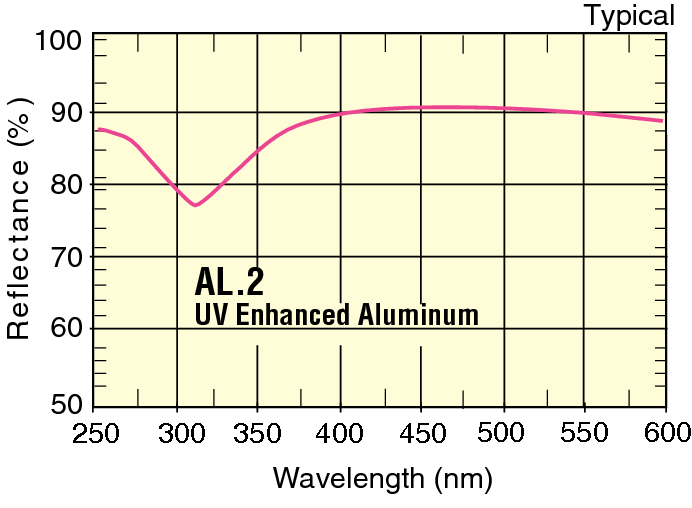
\includegraphics[width=1.0\linewidth]{images/Ref_Mirror}
    \caption{Typical mirror reference reflectivity  as specified by Newport.}
    \label{fig:Ref_Mirror}
\end{figure}
 
\subsection{Assembly and Tests of Half-Sector Mirrors}

The assembly of the half-sector mirrors was performed on the high-precision half-sector assembly table. The
assembly procedure had to ensure that there were no half-sector overlaps or gaps between half-sectors.
Figure~\ref{fig:Half-sector_assem_tb2} shows the table used for the assembly of all 12 half-sector mirrors. The
table was made of solid aluminum alloy block and has several features important for assembly with the required
accuracy:
\begin{itemize}
\item The overall dimensions of the working surface defined the overall dimensions of the half-sector mirror being
  assembled;
    \item The table was equipped with side plates on the left and right of each facet (8 plates total);
    \item The table was designed to be used for gluing of the facets to each other;
    \item The radial and transverse positions of the mirror could be controlled with accuracy up to 0.001~in by
      inserting spacers between the mirror facets and the side plates;
    \item Each of the 5 places for mounting the different mirror substrates functioned as a vacuum table with a
      spherical work surface, so that each  facet used in the assembly could  be put on the table and secured in place
      as needed by turning on the corresponding diaphragm vacuum pump;
    \item Along the edges of the adjacent mirrors that are in contact, the table has milled-out groves for collecting
      excess epoxy to prevent gluing of the facet to the table surface;
    \item Polymerization of the epoxy glue was possible to perform in a temperature and humidity-controlled
      environment;
    \item The table was part of the setup that allowed for geometry tests of the assembled half-sector.
\end{itemize}

\begin{figure}[ht]
    \centering
    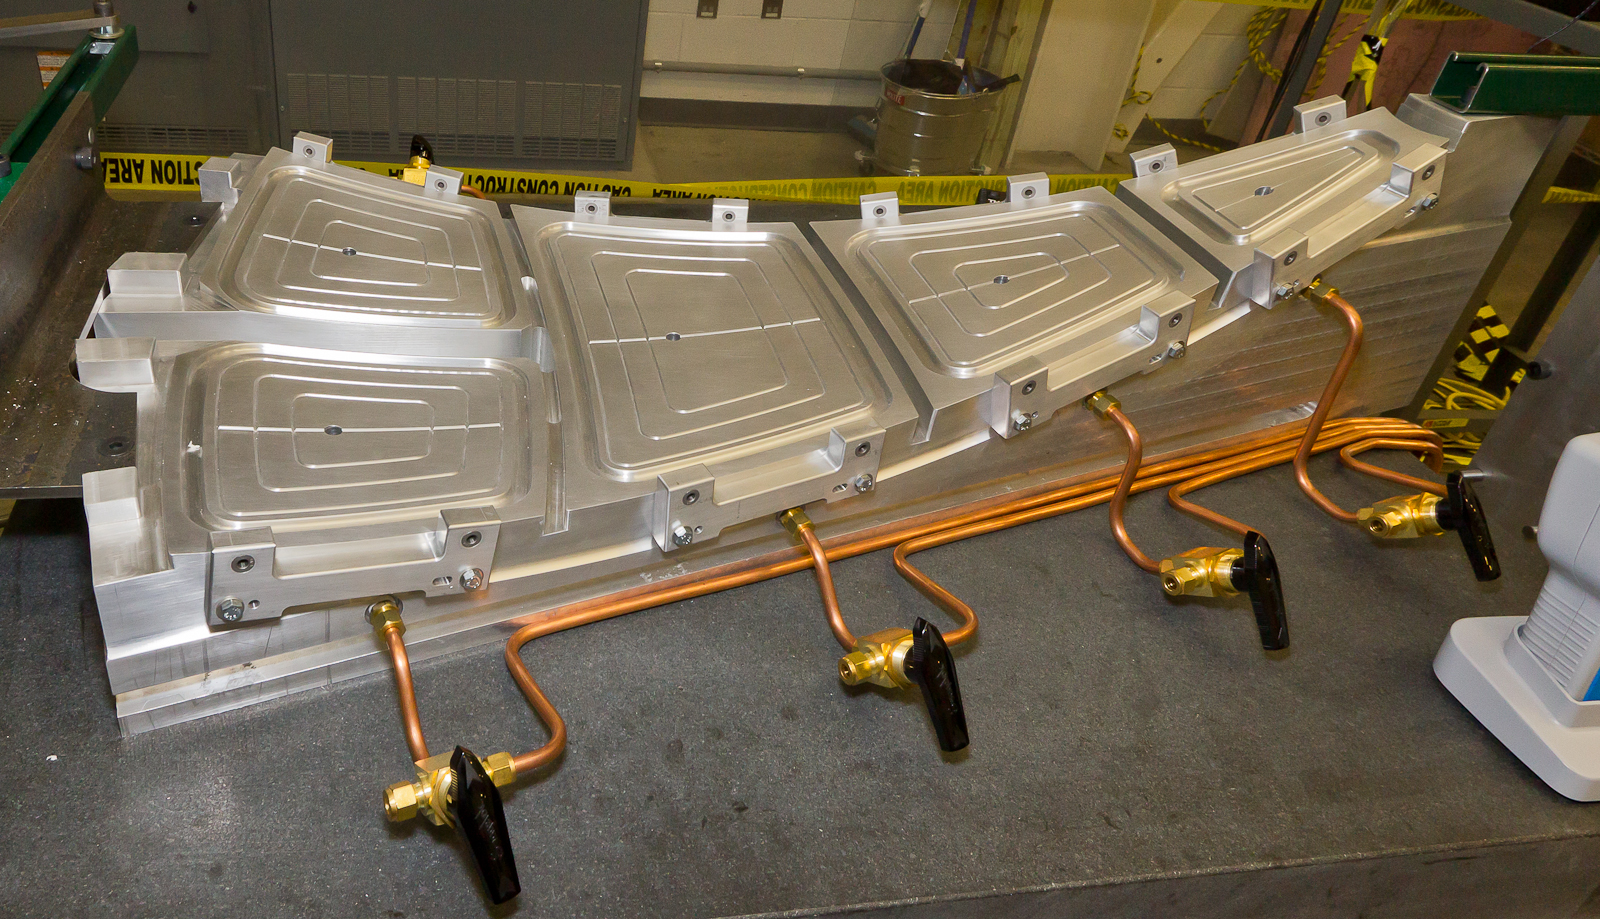
\includegraphics[width=1.0\linewidth]{images/Half-sector_assem_tb2.JPG}
    \caption{High-precision table for the assembly of the half-sector mirrors.}
    \label{fig:Half-sector_assem_tb2}
\end{figure}

The assembly of the combined mirror using location pins is preferable compared with side-to side direct gluing as
there are no deformations involved due to unavoidable epoxy glue shrinkage. Nevertheless, it was decided not to
use location pins since the thickness of the substrates (0.6 in) was relatively small and the mechanical strength of
the PMI foam that we used would introduce risks during final assembly, handling, and installation of the HTCC mirror.
Therefore we decided to directly glue the facets to each other. The gluing technique was based on applying the glue
in the form of dots uniformly distributed over the entire contact surface. The amount of glue in the dots and the
distance between them were such that the glue spots compressed between the facets did not touch each other. In
this case deformations caused by shrinkage of individual dots cancel each other and the shape of the final product
stays unchanged. The only dots that introduce uncompensated shrinkage deformation are near the edges of the glued
surfaces. The corresponding deformations do not change the mirror shape but they introduce a slight residual
waviness of the edges of the mirrors with a pattern that repeats as the pattern of dots. In fact the only concern was
to make sure the glue joints were strong enough. We ran comprehensive tests to come up with an acceptable solution
for using this kind of joint. We tried several different patterns of glue application, amount and viscosity of the glue,
applying glue on one side or both sides, etc. Figure~\ref{fig:Pattern} shows two identical foam pieces and the epoxy
application pattern used in the tests of the glue joint. 

\begin{figure}[ht]
    \centering
    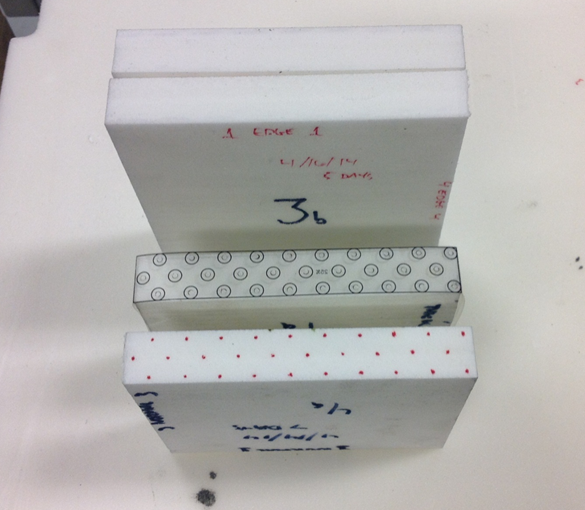
\includegraphics[width=1.0\linewidth]{images/Pattern.png}
    \caption{Foam pieces marked for an approximately 22.5\% epoxy coverage pattern.}
    \label{fig:Pattern}
\end{figure}

Standard Hysol epoxy with black pigment and 1:1 silica filler to epoxy by volume was applied as small dots (0.08-in
diameter). The viscosity of the epoxy filler mix was so thick that the glue did not bleed into the foam. 

Figure~\ref{fig:Glue_joint_test} shows the test setup to check the strength of the glue joint using two sample
substrate pieces. The epoxy cured for 72~hrs. The total force to break the glue joint was about 62~ft-lbs. The
force was applied evenly and the foam was torn from the glue on both test pieces, see Fig.~\ref{fig:Broken}. The
foam failed and not the glue itself. A set 0.004-in wide gap was left between the parts when gluing, and the glue
was directly applied to one piece only. When the bond failed it pulled out almost all of the glued dots evenly except
for the two places where the shims were set. The foam piece in Fig.~\ref{fig:Broken} that has the dots on it was
the same piece to which the epoxy was applied.

\begin{figure}[ht]
    \centering
    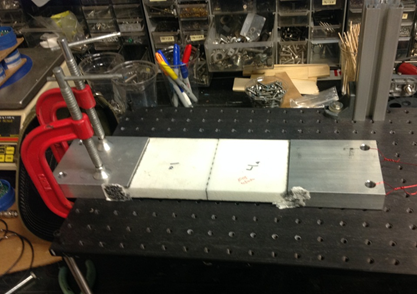
\includegraphics[width=0.95\linewidth]{images/Glue_joint_test.png}
    \caption{Test setup to check the strength of the substrate glue joint.}
    \label{fig:Glue_joint_test}
\end{figure}

\begin{figure}[ht]
    \centering
    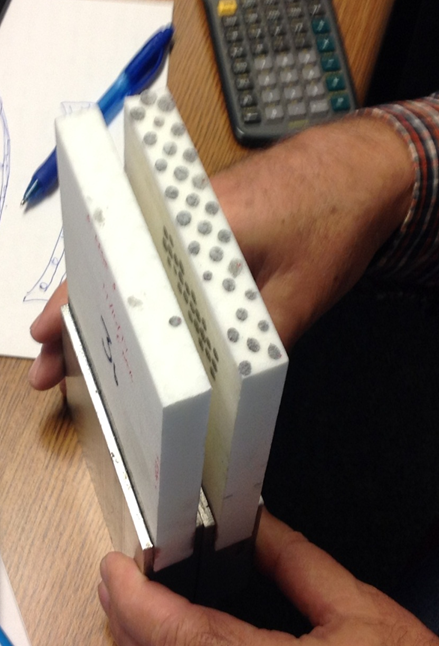
\includegraphics[width=1.0\linewidth]{images/Broken.png}
    \caption{Broken epoxy glue joint between two PMI foam pieces.}
    \label{fig:Broken}
\end{figure}

It has to be mentioned that the glue dots applied along the sides of the adjacent mirror facets will compensate
the shrinkage of each other that occurs after polymerization of the epoxy is completed. There are only two
uncompensated dots at the ends of any side to be glued. The effect of the shrinkage is too small because all other
dots along the glued sides are properly compensated and therefore the shape of the facet stays unchanged. 

%\begin{comment} Since along sides of any glued facets there are 3 to 4 rows of applied glue dots. Than the dots across
%  the width of the glued side are mostly not compensated. This directly leads to a certain deformation of edges of the
%  glued facets, i.e. the edge is still smooth line  but "wavy" and waviness pitch is defined by average distance between
%  adjacent glue dots. In other words the local light collection efficiency of the mirror facets along glued sides only
%  decreases since geometry of the edges are changed. It was possible to avoid this small decrease if more complicated
%  joint with location pins was used. Corresponding results obtained in the experiments with electron beam will yet be
%  discussed.
%\end{comment} 

The assembly of half-sectors was done step-by-step by placing mirror facets on the table starting from the smallest
mirror. The first facet once placed on the table was aligned and then checked for fit. After that the vacuum pump was
turned on to secure the mirror. It was impossible to shift the facet on the table by even a little bit without deforming
the mirror once the vacuum was established. The next step was to position the adjacent mirror with epoxy glue dots on
it into position in contact with the first mirror. Once aligned it was independently secured on the table using the same
vacuum pump. Epoxy glue dots were applied on the next facet and the procedure was repeated until the half-sector
was fully assembled. Figure~\ref{fig:Partial_Half-sector} shows a partially assembled half-sector mirror. The right
half (installed) and left half (yet missing) of the largest mirror have exactly the same geometry.

\begin{figure}[ht]
    \centering
    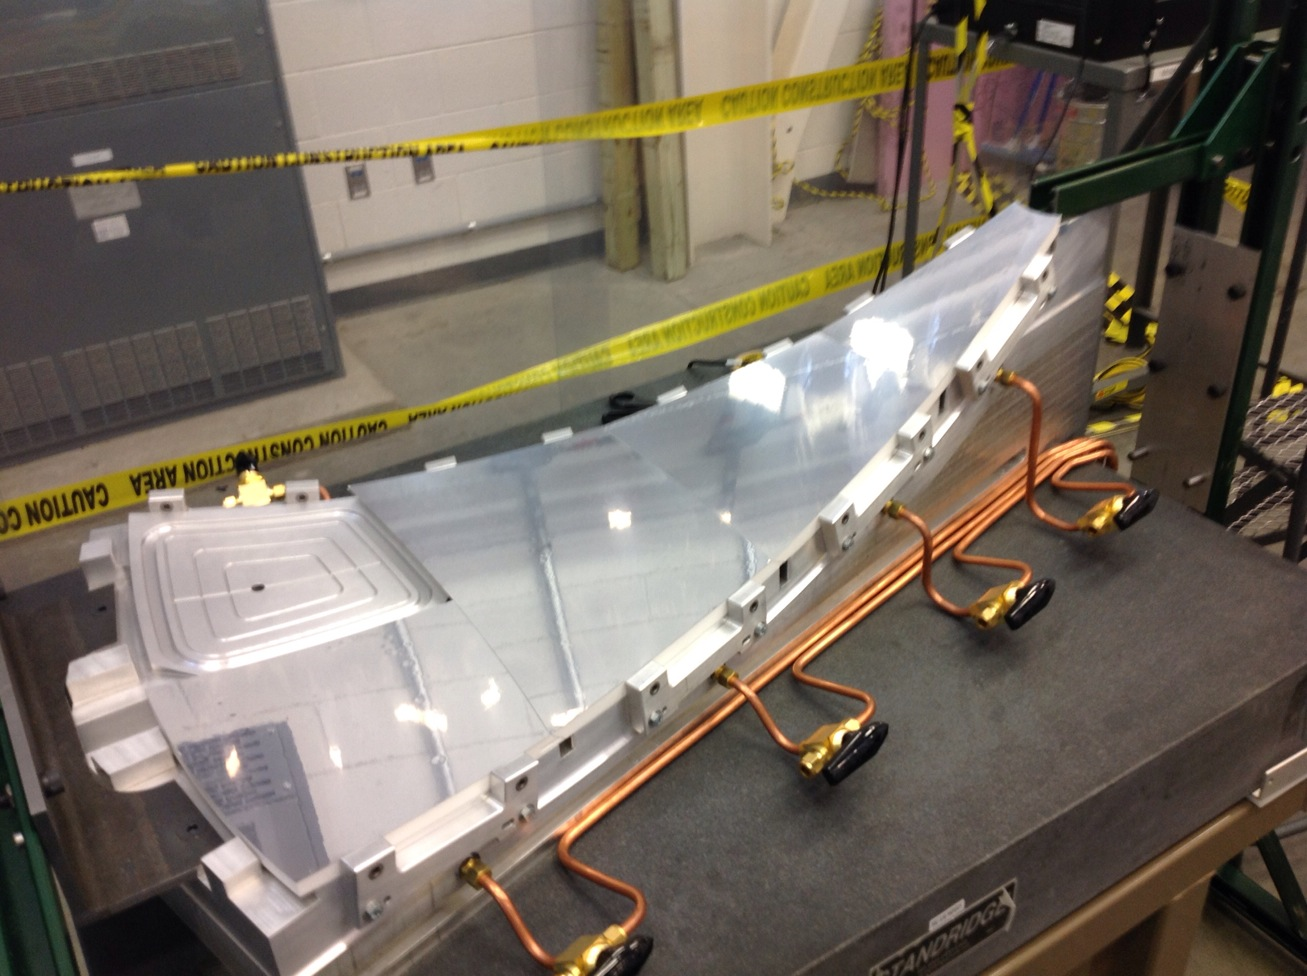
\includegraphics[width=1.0\linewidth]{images/Partial_Half-sector.png}
    \caption{Partially assembled half-sector mirror. The left facet of the last largest mirror is not installed yet.}
    \label{fig:Partial_Half-sector}
\end{figure} 

Figure~\ref{fig:Half-sector} shows a fully assembled half-sector mirror. It was left on the table under pressure
with vacuum pumps on for at least 24~hours or more depending on the polymerization results of the control glued
samples. 

\begin{figure}[ht]
    \centering
    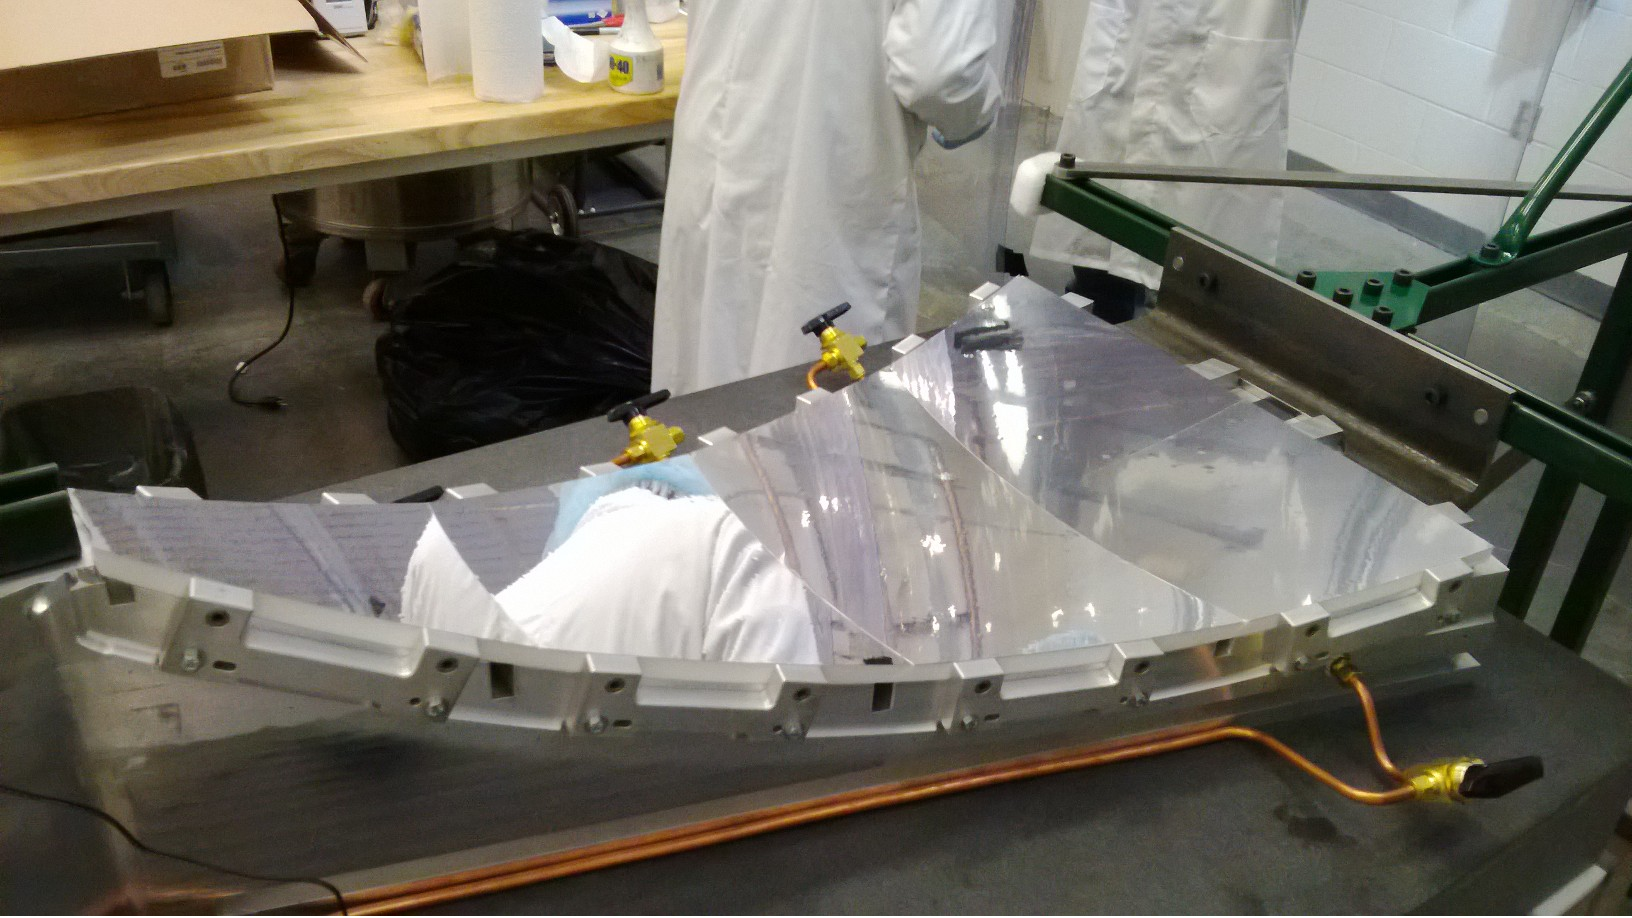
\includegraphics[width=1.0\linewidth]{images/Half-sector.png}
    \caption{Fully assembled half-sector mirror. The largest mirror consist of two mirror facets that have the same
      geometry.}
    \label{fig:Half-sector}
\end{figure}

The high-precision table was part of the half-sector mirror geometry test setup that was equipped with a
low-energy red laser, gimbal-mounted in the target position, and with four focal planes. The relative location of the
laser, assembly table, and focal planes were strictly defined by the designed geometry of the HTCC light collection.
The setup allowed for checking the actual geometry of light collection by each mirror using a point-like laser beam
as well as a beam rastered in the plane crossing any mirror over its entire surface. The light collection geometry
was checked on the half-sector mirrors after complete polymerization of the glue. The obtained pattern of the
light collection obtained on the focal plane of the smallest mirror facet that covers polar and azimuthal angles of
the scattering electrons in the range of $\theta = 5^\circ - 12.5^\circ$\, and\, $\phi = 0^\circ - 30^\circ$ is shown in
Fig.~\ref{fig:Focal_Plane_4}. The concentric circles on the focal plane are of diameter 1, 2, and 3~inches. Similar
results have been obtained for the remaining three mirror facets covering polar angular range of
$\theta = 12.5^\circ - 20^\circ$, $\theta = 20^\circ - 27.5^\circ$, and $\theta = 27.5^\circ - 35^\circ$. The
azimuthal angular coverage is the same for all facets. Figure~\ref{fig:Focal_Plane_1R} shows the light collection
pattern for the outermost, largest mirror facet. All 12 half-sector mirrors were assembled following exactly
the same procedures that allowed us to closely control the overall dimensions and therefore the values of the gaps
between adjacent half-sectors. 

\begin{figure}[ht]
    \centering
    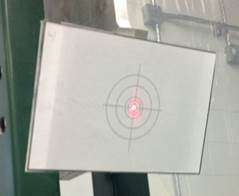
\includegraphics[width=0.90\linewidth]{images/Focal_Plane_4.jpg}
    \caption{Light collection pattern on the focal plane. The laser beam is rasterized in the plane crossing the mirror
      covering polar and azimuthal angles in the range of $\theta = 5^\circ - 12.5^\circ$\, and\,
      $\phi = 0^\circ - 30^\circ$.}
    \label{fig:Focal_Plane_4}
\end{figure}

%\begin{comment}
%\begin{figure}[ht]
%    \centering
%    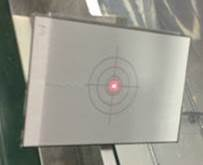
\includegraphics[width=0.90\linewidth]{images/Focal_Plane_3.jpg}
%    \caption{Light collection pattern on the focal plane for the mirror covering polar and azimuthal angles in the range
%      of $\theta = 12.5^\circ - 20^\circ$\, and\, $\phi = 0^\circ - 30^\circ$.}
%    \label{fig:Focal_Plane_3}
%\end{figure}
%
%\begin{figure}[ht]
%    \centering
%   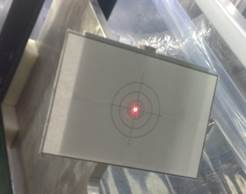
\includegraphics[width=0.94\linewidth]{images/Focal_Plane_2.jpg}
%    \caption{Light collection pattern on the focal plane for the mirror covering polar and azimuthal angles in the range
%      of $\theta = 20^\circ - 27.5^\circ$\, and\, $\phi = 0^\circ - 30^\circ$.}
%    \label{fig:Focal_Plane_2}
%\end{figure}
%\end{comment}

\begin{figure}[ht]
    \centering
    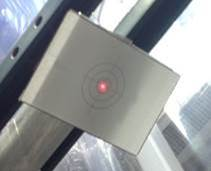
\includegraphics[width=0.95\linewidth]{images/Focal_Plane_1R.jpg}
    \caption{Light collection pattern on the focal plane for the mirror covering polar and azimuthal angles in the range
      of $\theta = 27.5^\circ - 35^\circ$\, and\, $\phi = 0^\circ - 30^\circ$.}
    \label{fig:Focal_Plane_1R}
\end{figure}

\subsection{Assembly of the Combined Mirror}

The combined HTCC mirror was assembled based on the experience acquired during the final assembly of the
half-sector mirrors. In order to do this we designed and built the half-sector mirror vacuum holding table for
assembly of the combined mirror. The design of this table and the accuracy of its manufacturing and construction
were critical in providing the required parameters of the combined mirror, such as the geometry of the mirror
optics, the stability of its shape, and its mechanical integrity. A peculiar feature of the combined HTCC mirror is
that it had to provide the correct light collection geometry for all 60 of its mirror facets glued together. The
option of making even very small adjustments of individual facets was excluded by the design.
 
For final mirror assembly we had to build 12 identical half-sector assembly tables and put them together due to the
relatively large overall dimensions of the HTCC mirror. The only difference between the high-accuracy half-sector
assembly table and the 12 identical tables for the final assembly was that they did not have the side plates.
Figure~\ref{fig:One_Foam_Vacuum_Table} shows one of the 12 vacuum tables made of medium density
polyurethane foam with 100\% closed cells.
 
\begin{figure}[ht]
    \centering
    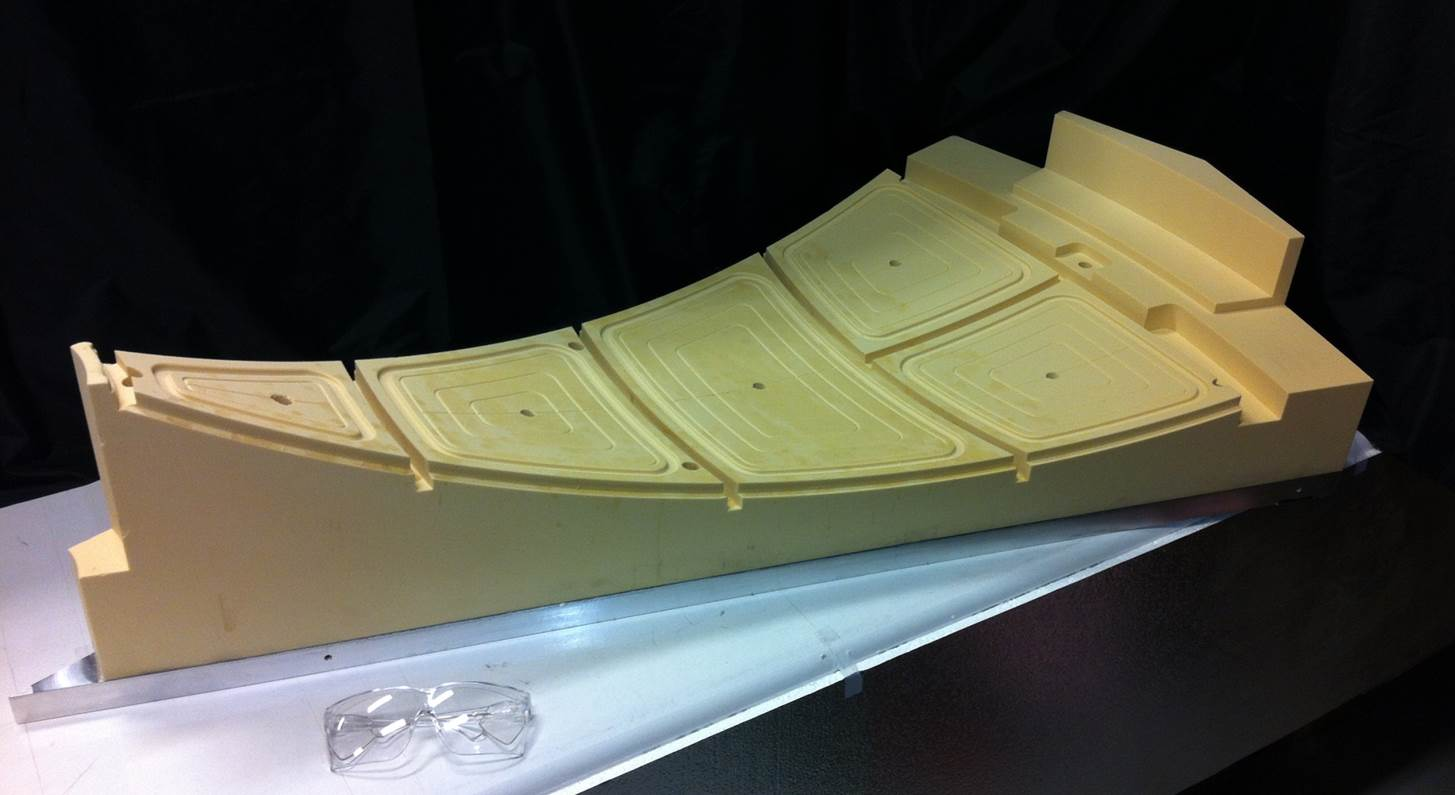
\includegraphics[width=1.0\linewidth]{images/One_Foam_Vacuum_Table.jpg}
    \caption{One of the 12 polyurethane half-sector holding tables.}
    \label{fig:One_Foam_Vacuum_Table}
\end{figure}
 
The top portion of the table is made of one solid block of polyurethane foam. It is glued to a 1-in thick wedge-shaped
flat aluminum plate. To avoid or minimize possible warping we used plates of 1100 aluminum alloy. The smoothness and
accuracy of manufacturing the top surface of the table ensured the ability of the table to firmly hold the half-sector
mirror. No gaskets of any kind were used to enhance the holding ability of the table. On the working surface of the
vacuum table there are five independent circular grooves through which air is pumped out under each of the five
mirror facets of the half-sector mirror. 

%\begin{comment}
%  Six vacuum foam tables fully assembled on one of identical 1 inch plates are shown on the
%  Fig.~\ref{fig:Six_Foam_Vacuum_Tables}.
% 
%\begin{figure}[ht]
%    \centering
%    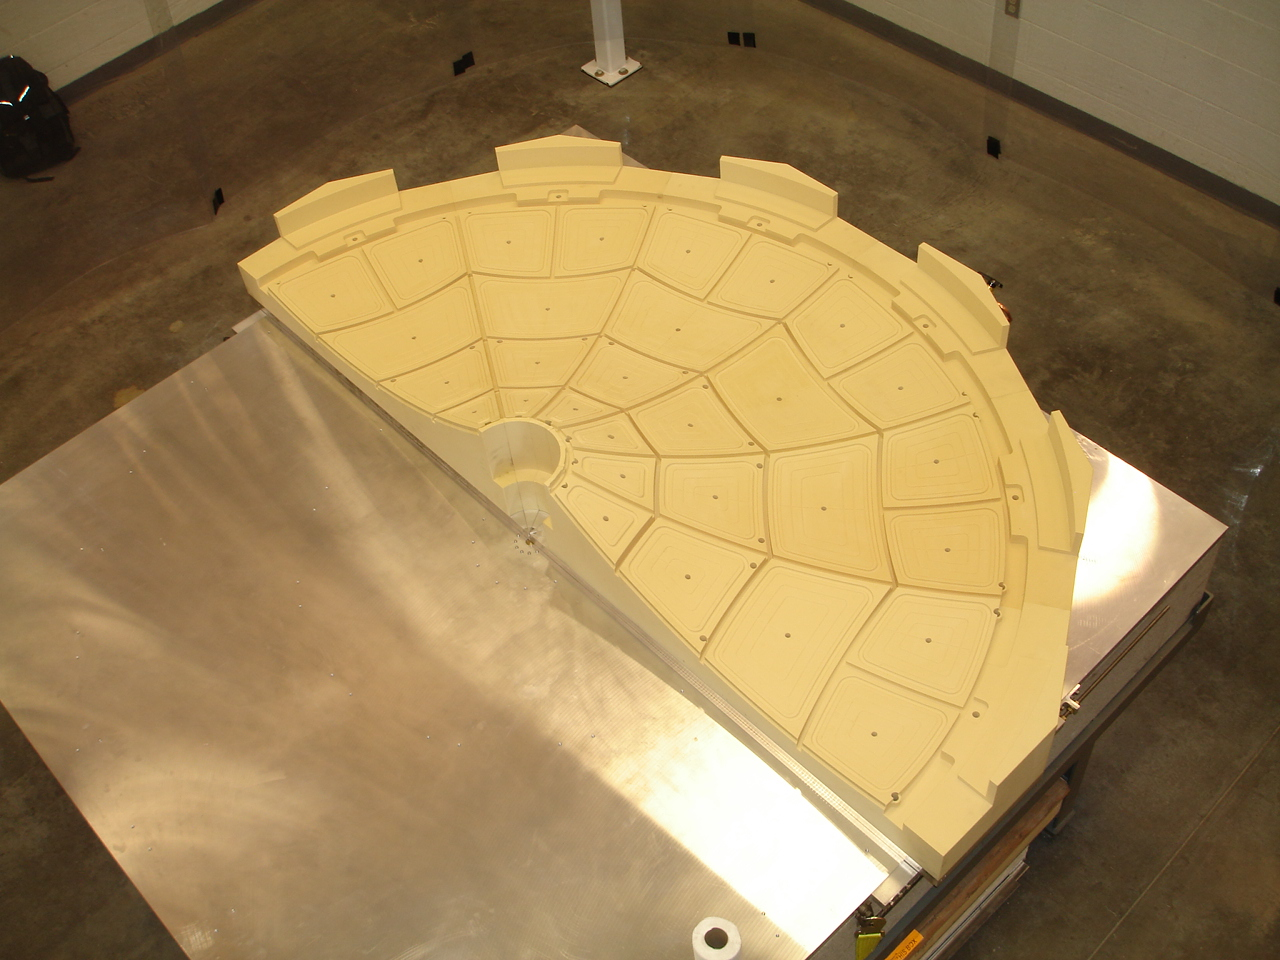
\includegraphics[width=1.0\linewidth]{images/Six_Foam_Vacuum_Tables.jpg}
%    \caption{Six half-sector holding vacuum tables assembled on the 1 inch aluminum plate placed on the granite table}
%    \label{fig:Six_Foam_Vacuum_Tables}
%\end{figure}
%\end{comment}

The entire set of 12 half-sector vacuum holding tables was assembled on two identical 1-in thick flat plates
carrying 6 tables each. These plates were mounted and aligned on the top of a 10~ft by~10 ft granite table.
Fig.~\ref{fig:Twelve_Foam_Vacuum_Tables} shows the vacuum table for the assembly of the combined HTCC
mirror fully equipped with the 60 pumping control valves (5 valves per half-sector). We had to provide tight
ambient control (dust level, temperature, and humidity). The table was also equipped with a transparent hood (not
shown in Fig.~\ref{fig:Twelve_Foam_Vacuum_Tables}) to cover the entire table to run tests at different relative
humidity.   

\begin{figure}[ht]
    \centering
    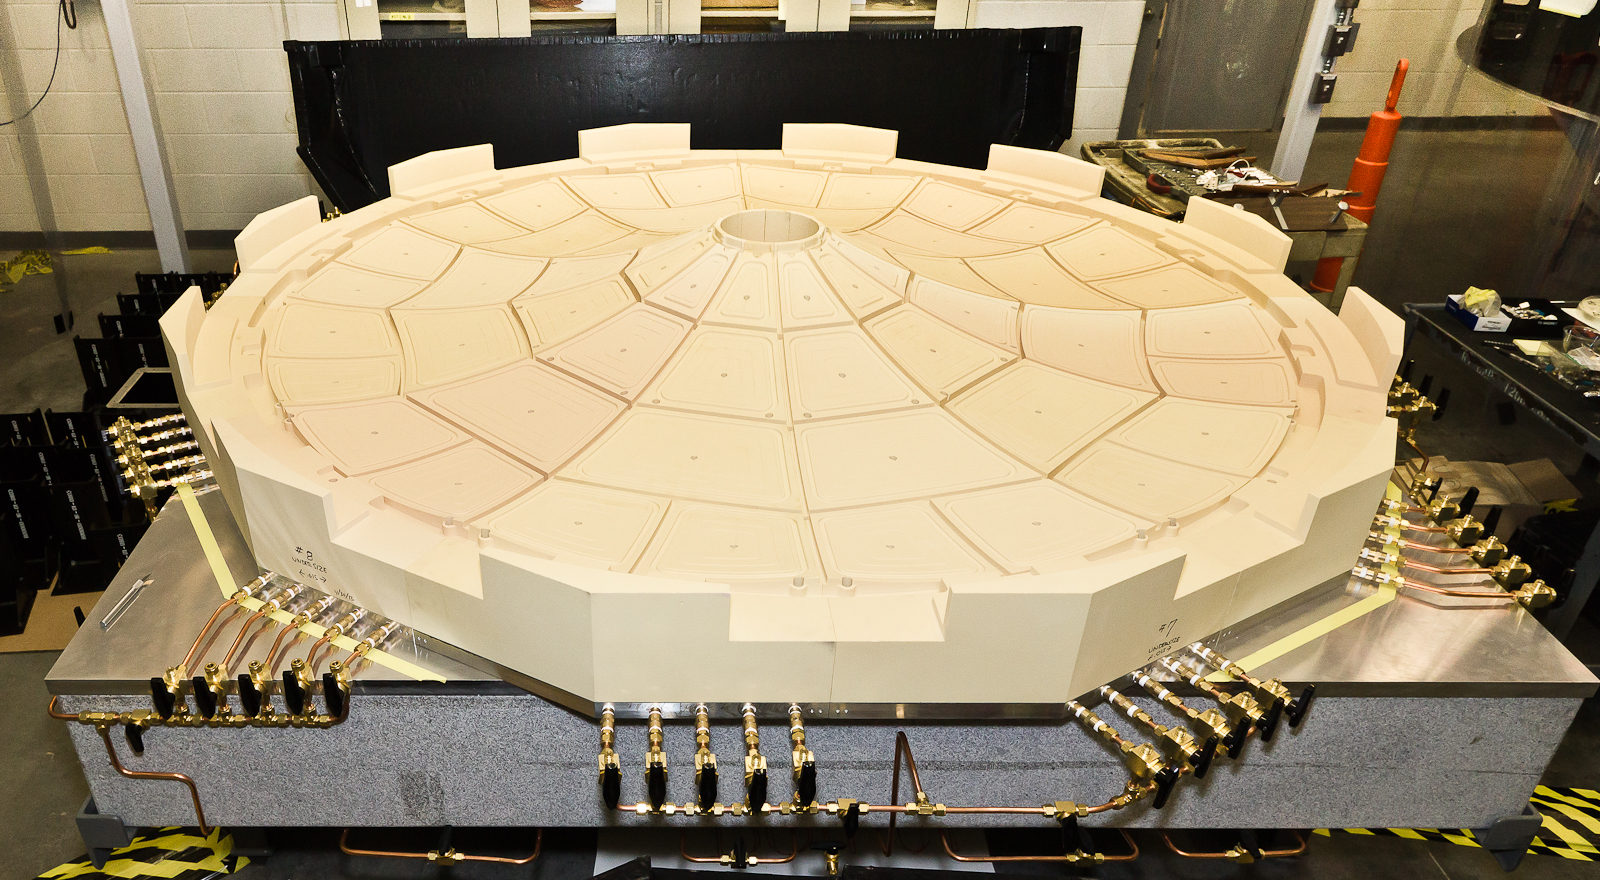
\includegraphics[width=1.0\linewidth]{images/Twelve_Foam_Vacuum_Tables.jpg}
    \caption{All 12 half-sector vacuum tables assembled on their 1~in aluminum plates placed on the granite table.}
    \label{fig:Twelve_Foam_Vacuum_Tables}
\end{figure}

It was decided not to equip the table with any devices to check the geometry of the HTCC mirror during assembly.
Since the 12 assembled half-sectors passed tight quality controls, there was not much room available for adjustment
of the half-sectors on the final assembly table within more than about 0.030~in in the radial direction and within gaps
between adjacent half-sectors of about 0.010~in. The geometry was essentially established and fixed once all 12
half-sectors were held tight on the table.

The assembly procedure was the same used before for the half-sectors. The only difference was that we had to
install in the center of the combined mirror the light-weight central ring (0.055-in thick) made of carbon fiber.
The ring was glued to all half-sectors. We controlled and measured the gaps between all adjacent mirror facets
belonging to adjacent half-sectors. The average gap was 0.0096~in and is very close to the design value of
0.008~in, which represents the ``dead" zone between the half-sectors. The HTCC covers almost 100\% of the
azimuthal angular acceptance of the CLAS12 Forward Detector. It has to be mentioned that the average gaps
between adjacent facets in the given half-sector mirror were 50\% smaller, which provides very compact coverage
in the polar angle. 

The final assembly of the combined HTCC mirror started with applying the epoxy glue on the first half-sector as
shown in Fig.~\ref{fig:Ap_Gl_Half_Sect}, using the same procedure employed for the assembly of the
half-sectors. Figure~\ref{fig:Partial_Assembl_MIR} shows the partially assembled combined mirror and 
Fig.~\ref{fig:Compl_Assembl_MIR} shows the completed mirror. 
 
\begin{figure}[ht]
    \centering
    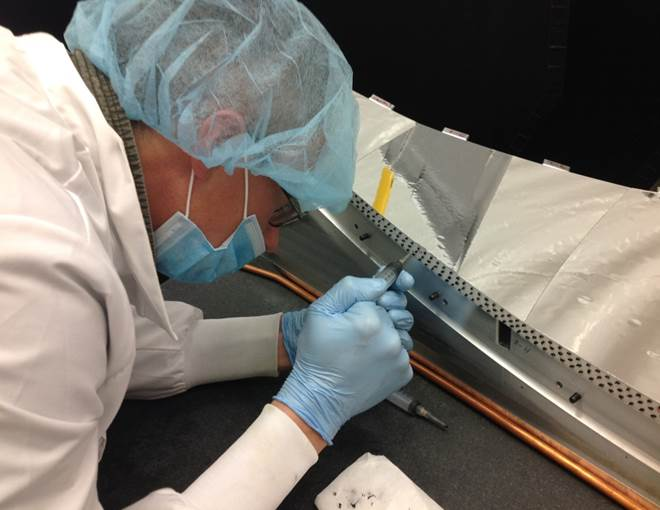
\includegraphics[width=1.0\linewidth]{images/Ap_Gl_Half_Sect.jpg}
    \caption{The dots of epoxy glue being applied to only one side of the half-sector mirror assembly.}
    \label{fig:Ap_Gl_Half_Sect}
\end{figure}
 
 \begin{figure}[ht]
    \centering
    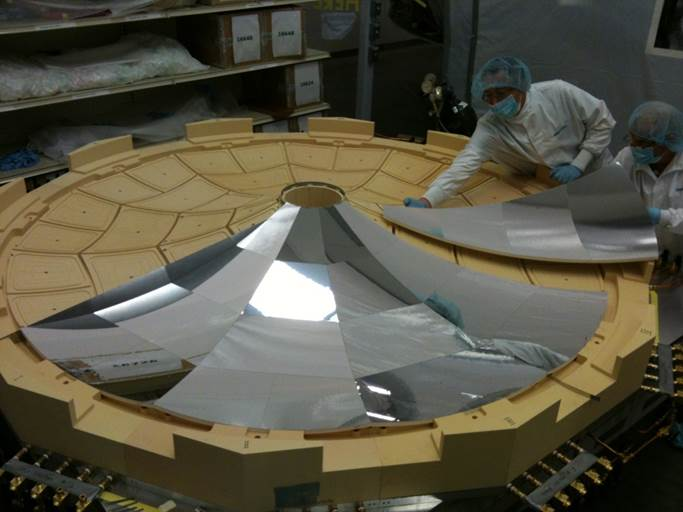
\includegraphics[width=1.0\linewidth]{images/Partial_Assembl_MIR.jpg}
    \caption{ Partially assembled combined HTCC mirror.}
    \label{fig:Partial_Assembl_MIR}
\end{figure}

 \begin{figure}[ht]
    \centering
    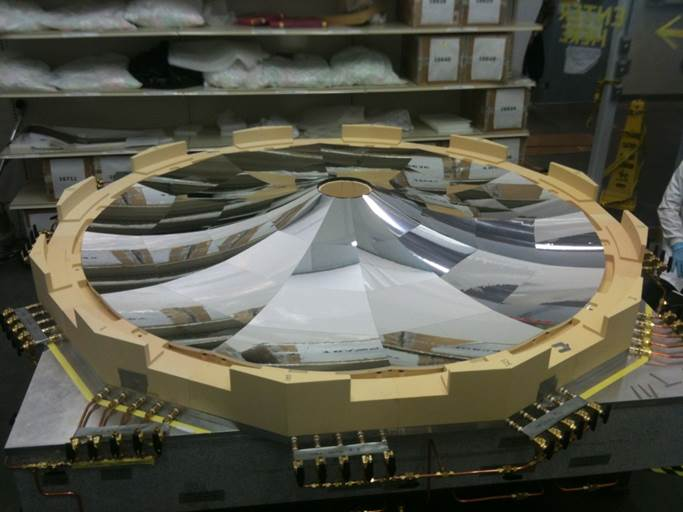
\includegraphics[width=1.0\linewidth]{images/Compl_Assembl_MIR.jpg}
    \caption{Fully Assembled combined HTCC mirror.}
    \label{fig:Compl_Assembl_MIR}
\end{figure}

We used a special procedure to glue the last half-sector because otherwise we would have had to insert the last
half-sector in a very narrow space that would have smeared the glue dots. Therefore, we assembled the first 6
half-sectors on the first 1-in mounting plate, and the remaining 6 half-sectors on the other 1-in mounting plate.
The mounting plates with the 6 half-sectors were positioned on the granite table leaving a gap about 1 in wide,
(see Fig.~\ref{fig:Separated_halves}). Epoxy glue was then applied to the one of the exposed sides, (see
Fig.~\ref{fig:Final_Gluing}), and the plates were slid together so that both sides come in contact.
 
  \begin{figure}[ht]
    \centering
    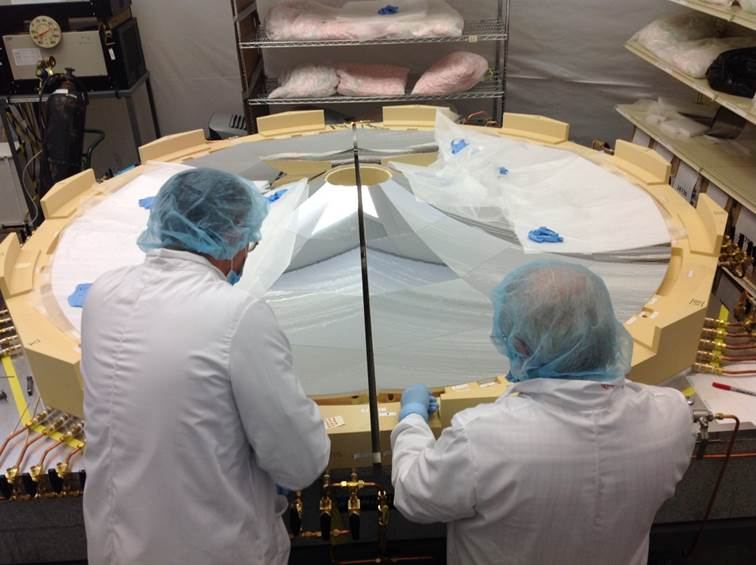
\includegraphics[width=1.0\linewidth]{images/Separated_halves.jpg}
    \caption{Separated halves of the combined mirror before final gluing.}
    \label{fig:Separated_halves}
\end{figure}
         
 \begin{figure}[ht]
    \centering
    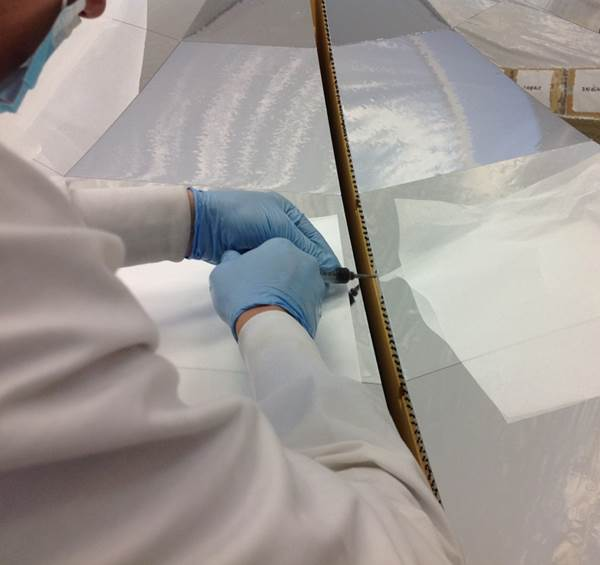
\includegraphics[width=1.0\linewidth]{images/Final_Gluing.jpg}
    \caption{Application of the epoxy glue on the side of the separated halves of the combined mirror.}
    \label{fig:Final_Gluing}
\end{figure}
  
All elements that support and hold the combined mirror are out of the acceptance of the HTCC, see
Fig.~\ref{fig:Support_Ring}. The rigid, light-weight, composite supporting ring (strong-back) was attached to the
combined mirror via 12 composite light-weight bridge pieces glued to the side around of the mirror. The completely
assembled HTCC mirror, ready for installation, is shown in Fig.~\ref{fig:Ring_to_Mirror}. Since the rigidity of the
supporting parts is much higher than the rigidity of the combined mirror, we used flexible silicon compound for
gluing.
  
\begin{figure}[ht]
    \centering
    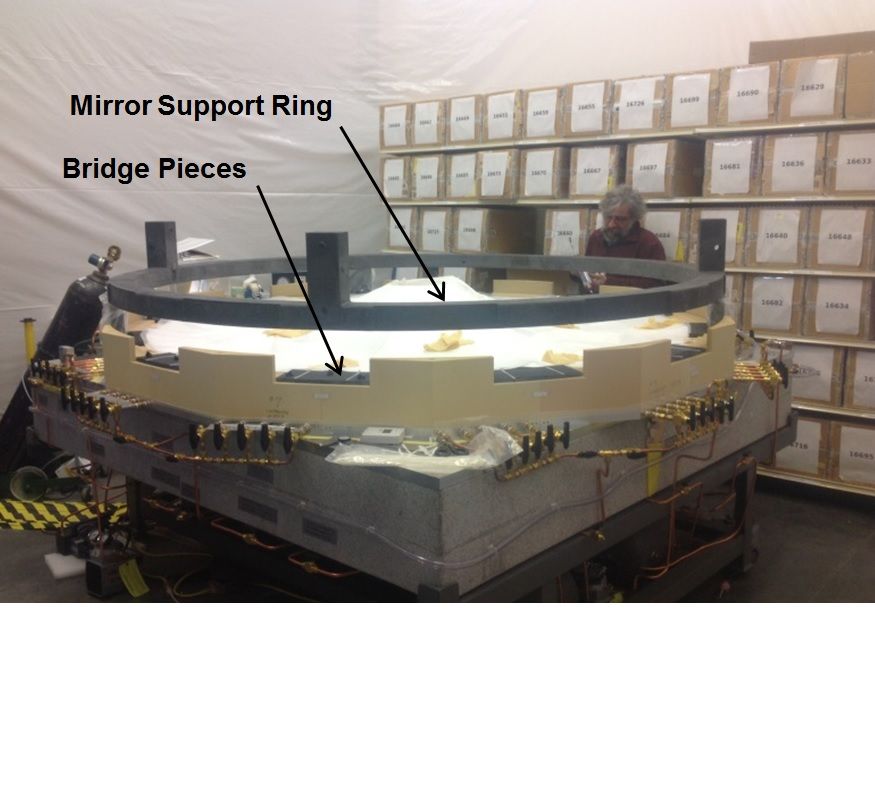
\includegraphics[width=1.0\linewidth,trim={0 5cm 0 0},clip]{images/Support_Ring.jpg}
    \caption{Supporting elements ready to be attached to the combined mirror. The mirror is covered with soft paper
      towels to protect the working surface from debris.}
    \label{fig:Support_Ring}
\end{figure}

\begin{figure}[ht]
    \centering
    %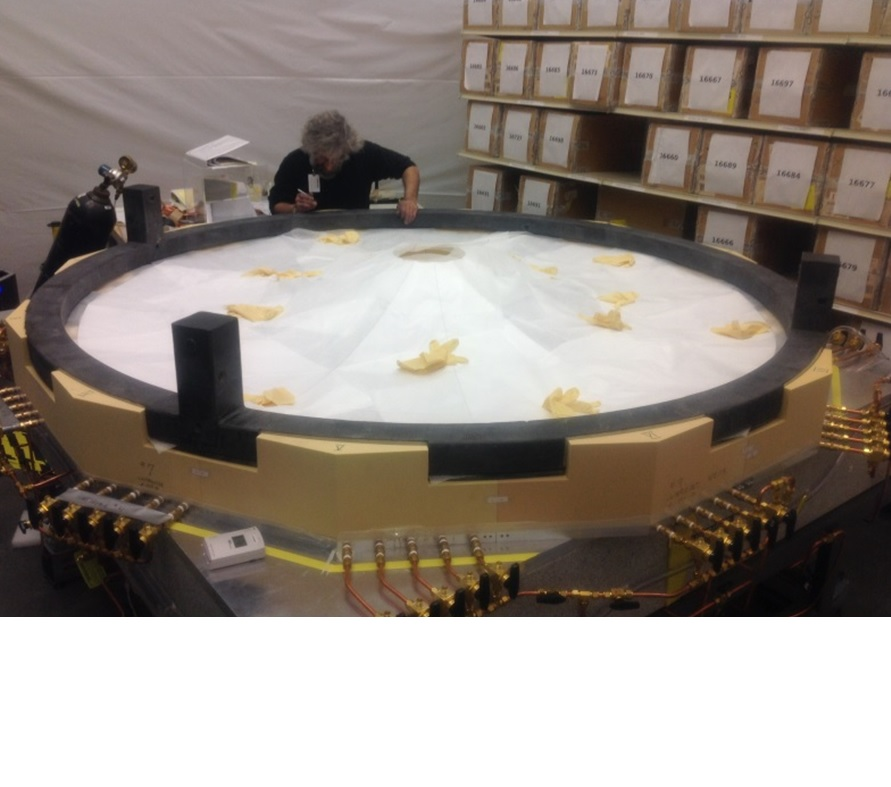
\includegraphics[width=1.0\linewidth,trim={0 5cm 0 0},clip]{images/Ring_to_Mirror.jpg}
    %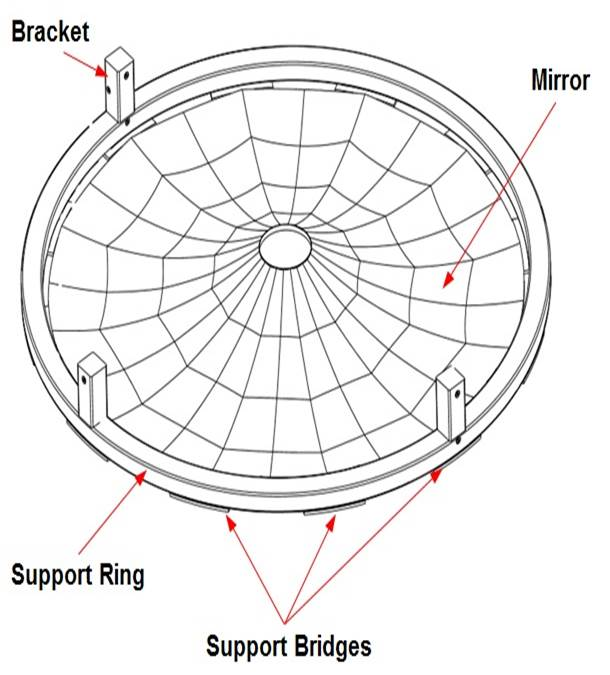
\includegraphics[width=1.0\linewidth,trim={0 5cm 0 0},clip]{images/Support_Ring_2.jpg}
        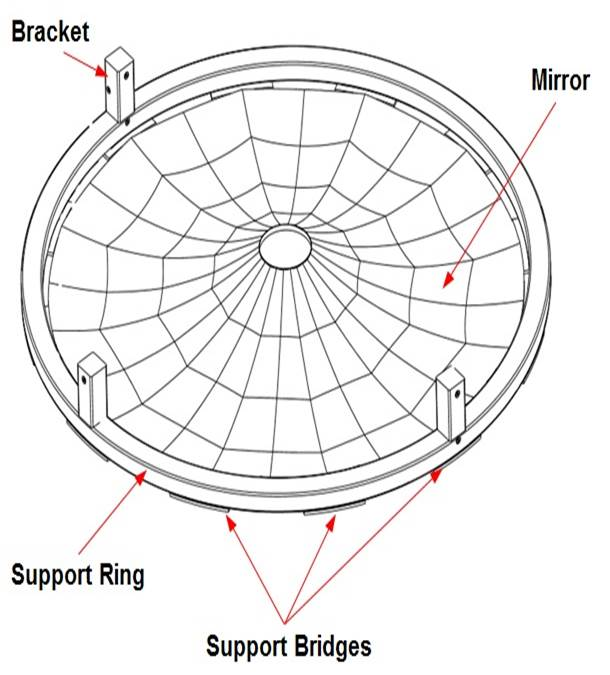
\includegraphics[width=1.0\linewidth]{images/Support_Ring_2.jpg}
    \caption{Completely assembled HTCC mirror ready for installation.}
    \label{fig:Ring_to_Mirror}
\end{figure}
 
\subsection {Entry and Exit Windows}

There are several aspects that have been taken into consideration that define the design of the entry and
exit windows:

\begin{itemize}
    \item Large area to cover;
    \item Small thickness;
    \item Opaque;
    \item High durability;
    \item Attachment to the main frame;
    \item Structural stability, i.e. resistance to pressure variations.
    \end{itemize}

The entry and exit windows are composite films made of three layers laminated together: Tedlar (thickness
38~$\mu$m), Mylar (thickness 75~$\mu$m), Tedlar (38~$\mu$m). The composite films came in rolls 61~in
wide. To make the exit window, three composite films were glued together side by side. The glue joint between
adjacent composite films was made in such a way that the thickness of the joint exceeded the remaining portions
by no more than 10\%. The usage of two black Tedlar films in the composite window guaranteed light insulation
even if one layer had any holes. One layer of Mylar film provided excellent durability and flexibility.

The dimensions of the entry and exit windows are $\approx$2.5~ft and $\approx$9.5~ft, respectively, so the
difference is significant. This required developing a special design for their attachment to the body of the
detector. The primary electron beam passes through the HTCC exactly along the axis of the detector. To
decrease the background of M{\o}ller electrons we have used a long shielding piece made of tungsten around
the beam that nominally covers polar angles up to 2$^\circ$ and has a small cylindrical opening in the center that
goes all the way through and is big enough for the beam~\cite{beamline-nim}. The volume of the HTCC must be
separated from the volume occupied by the tungsten metal shield. Since the corresponding HTCC part called the
M{\o}ller Cup that is concentric with the tungsten absorber must be light-weight, the joints between this part and
the entry and exit windows must also be light-weight. In this case, since the windows have different dimensions, any
changes in atmospheric pressure would cause both windows and the M{\o}ller Cup attached to them to move upstream
or downstream - depending on atmospheric pressure changes. The mirror could be damaged by the exit window if the
pressure goes up, or it could be damaged by the conical M{\o}ller  Cup if the pressure goes down (see
Fig.~\ref{fig:side_view}). Thus the M{\o}ller Cup has to be kept in the same location relative to the mirror
regardless of the fluctuations in atmospheric pressure. Even small changes of $\sim$1~mm of Hg would generate
a force of $\sim$200~lbs acting on the M{\o}ller Cup along its axis.  

\begin{figure}[ht]
    \centering
    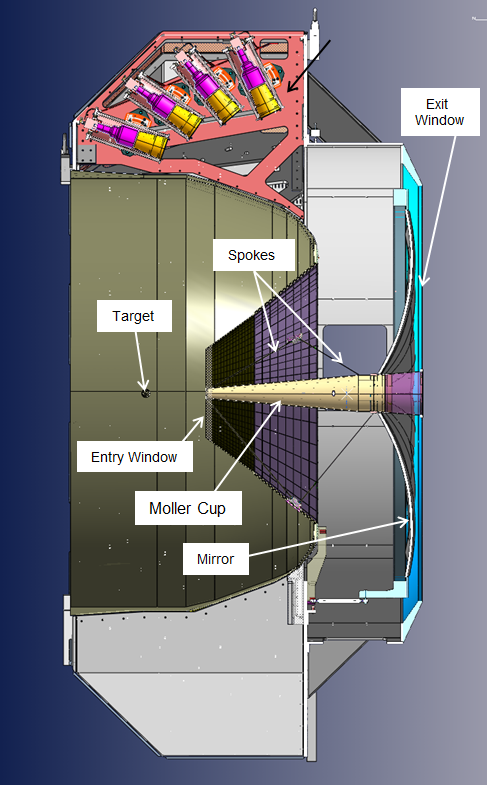
\includegraphics[trim={1.5cm 5cm 0 2cm }, clip, width=\linewidth]{images/Spokes2.png}
    \caption{Side view of the HTCC. The  entry and exit windows are shown along with other internal components.
    The beam is incident from the left.}
    \label{fig:side_view}
\end{figure}

To avoid potential problems with the integrity of the detector, the M{\o}ller Cup was attached to the main frame
of the HTCC at 12 points: 6 points on the upstream portion of the main frame, and the remaining 6 points on the
downstream portion. All parts providing attachments of the M{\o}ller Cup to the front or to the back of the main
frame are completely located in the shadow zone of the 6 superconducting coils of the torus magnet
\cite{magnets-nim}, i.e. they do not create any obstruction to the particles going through the drift chambers. The
M{\o}ller Cup was attached using 12 thin spokes, each 1.5~mm in diameter and was made of carbon fibers to minimize
the possible scattering of particles traveling within the shadow of the torus coils. The spokes very firmly hold the
M{\o}ller Cup in position. Each of them were tensioned as necessary to provide structural rigidity and to withstand
the stresses generated by the attached windows during atmospheric pressure changes. They were tensioned as a
string in order to eliminate any possible damage due to deformations of the body of the HTCC while
transporting, installing, or aligning. Each spoke is spring-loaded from both ends. Fig.~\ref{fig:Front_View} and
Fig.~\ref{fig:Exit_Win} show the upstream and downstream views of the HTCC with the entry and exit windows
installed.

\begin{figure}[ht]
    \centering
    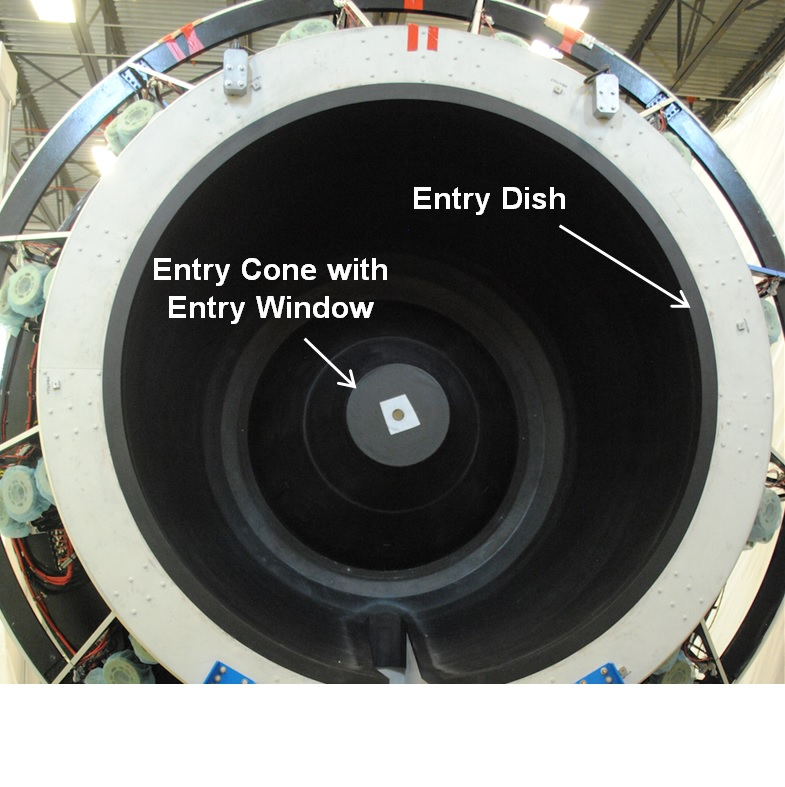
\includegraphics[width=1.0\linewidth,trim={0 2.5cm 0 0},clip]{images/Front_View}
    \caption{Upstream view of the HTCC.}
    \label{fig:Front_View}
\end{figure}

\begin{figure}[ht]
    \centering
    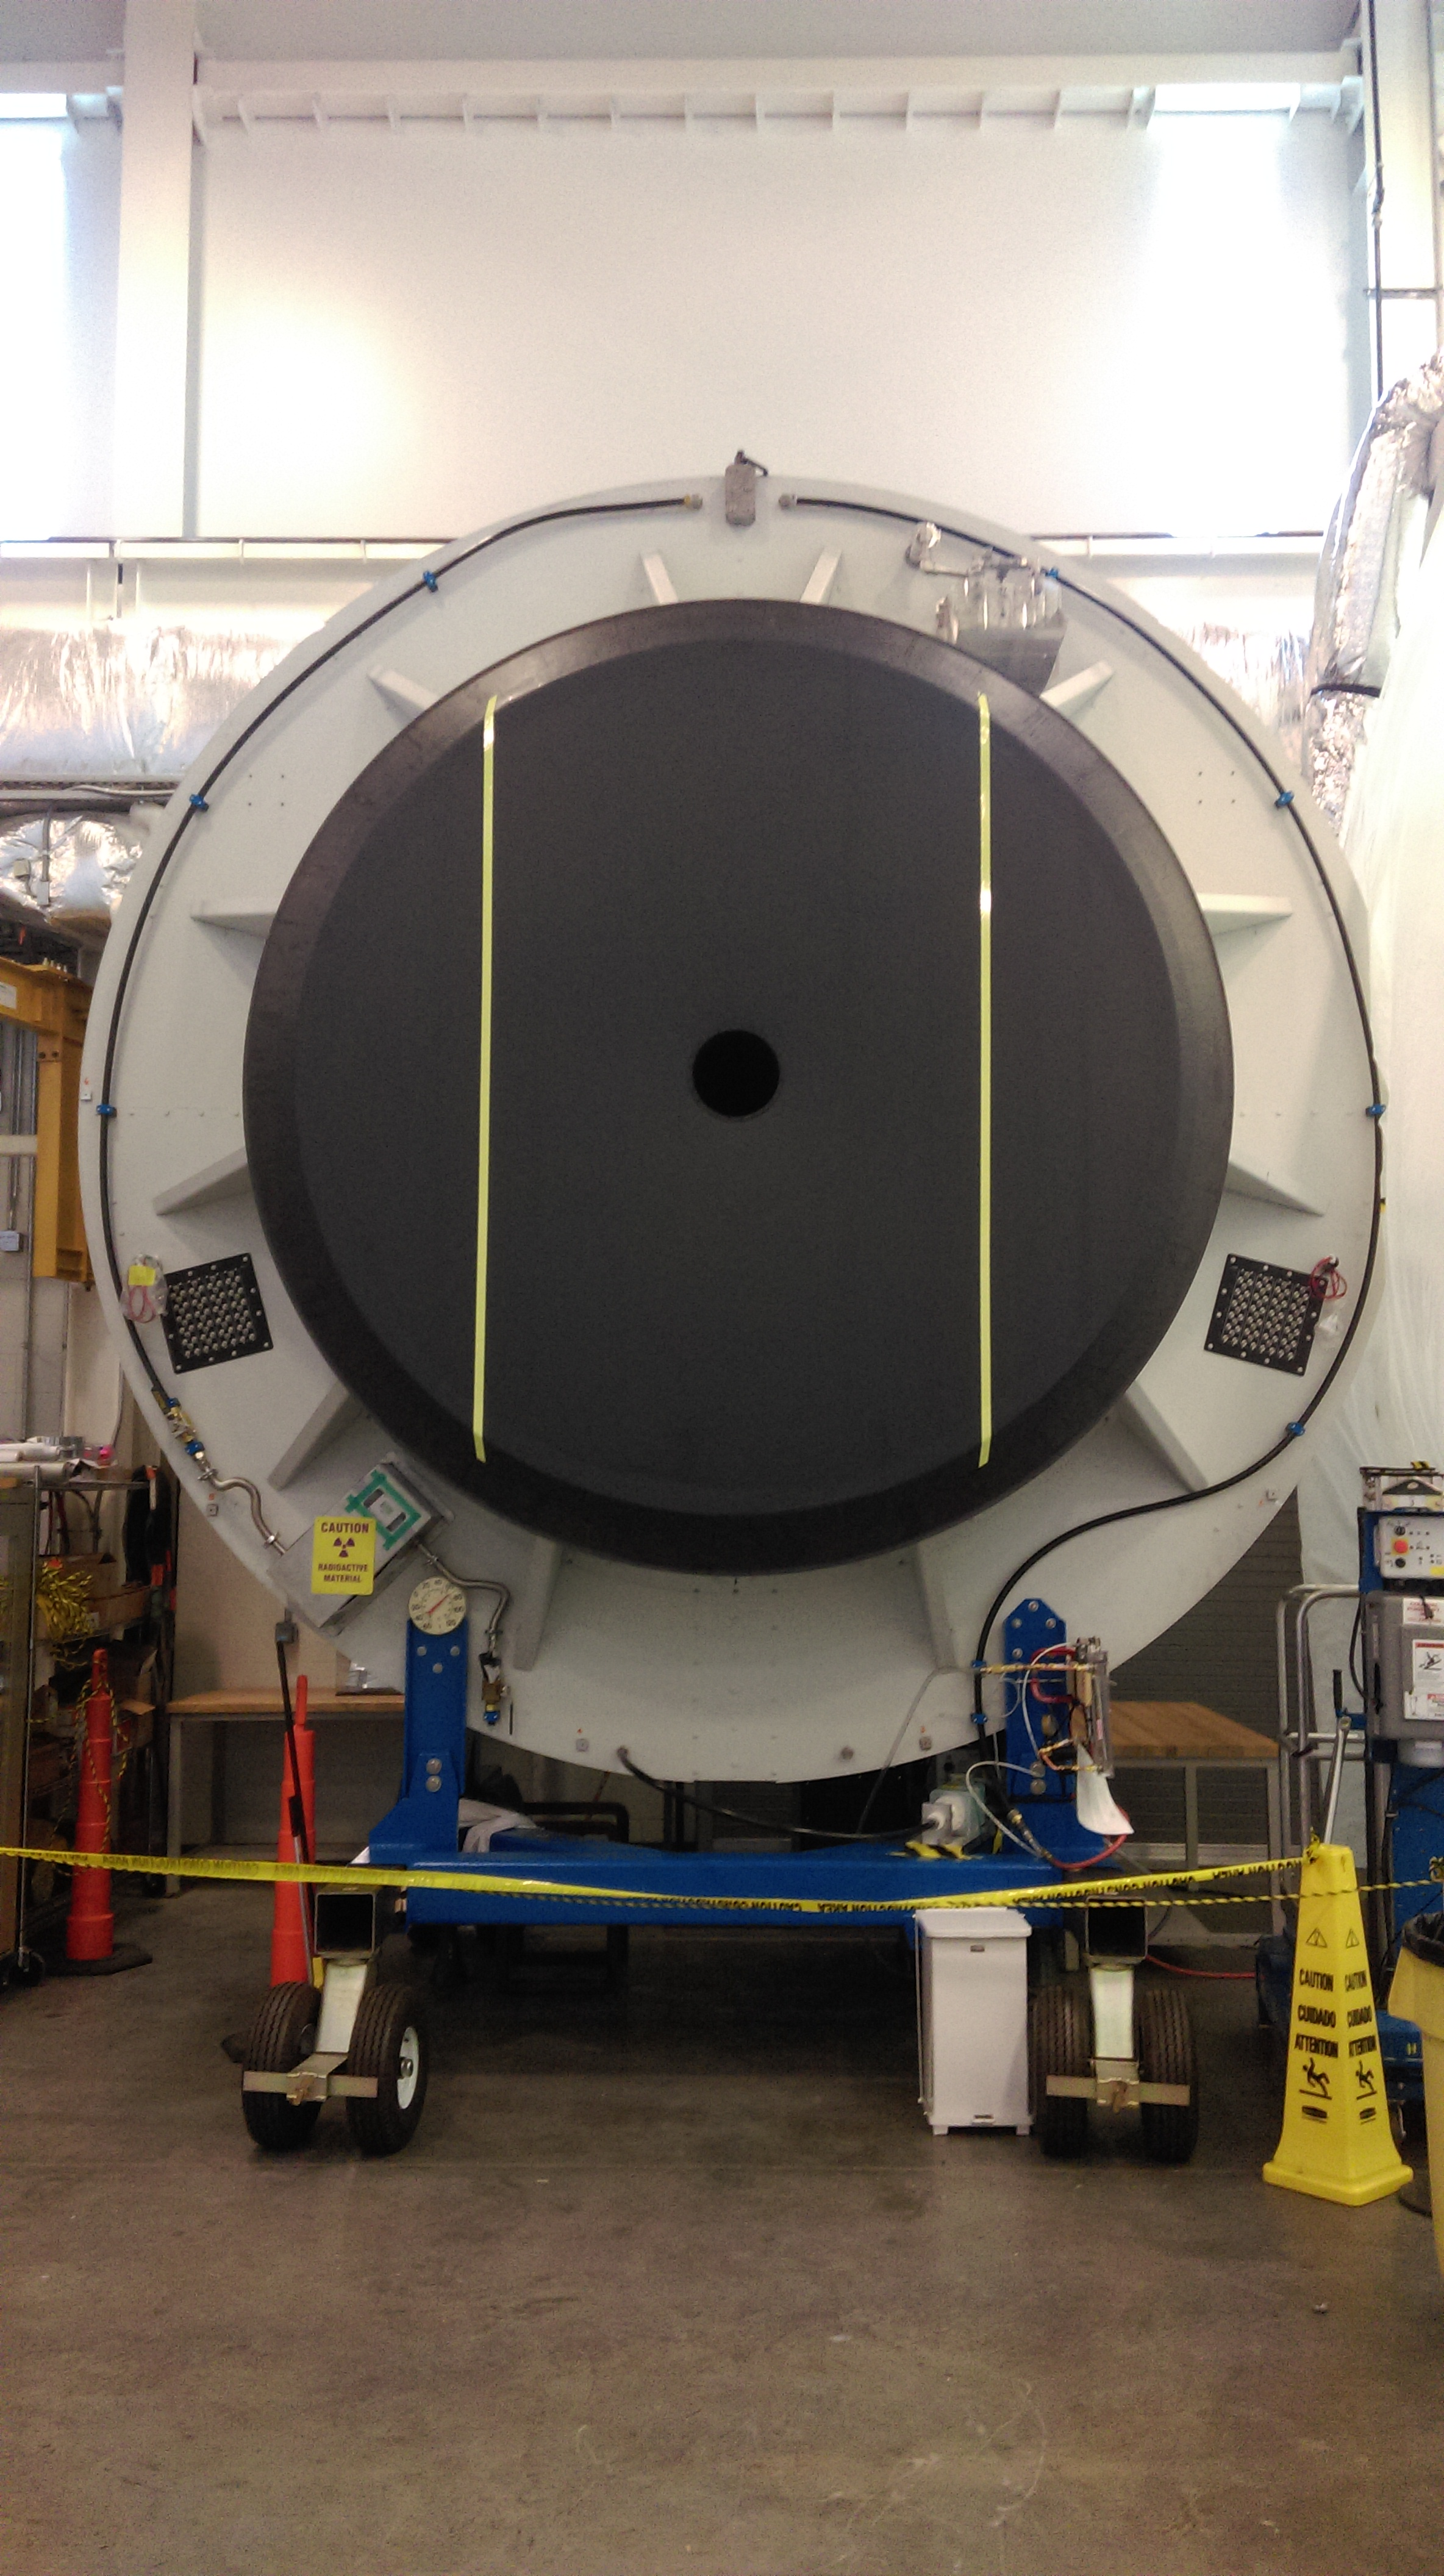
\includegraphics[width=1.0\linewidth,trim={0 25cm 0 500},clip]{images/Exit_Win.jpg}
    \caption{Downstream view of the HTCC.}
    \label{fig:Exit_Win}
\end{figure}

\subsection{Containment Vessel and Combined Mirror Installation}

The HTCC Containment Vessel has properties to satisfy a number of requirements, which included the safe
transportation of the fully assembled HTCC to the experimental hall without any changes in the alignment of the
internal components and the preservation of the mirror integrity. We tested the integrity of the spare mirror by
transporting it along the chosen route (see Fig.~\ref{fig:transportation_spare_mirror}), and successfully
transported the detector using the results obtained during the test. 

\begin{figure}[ht]
    \centering
    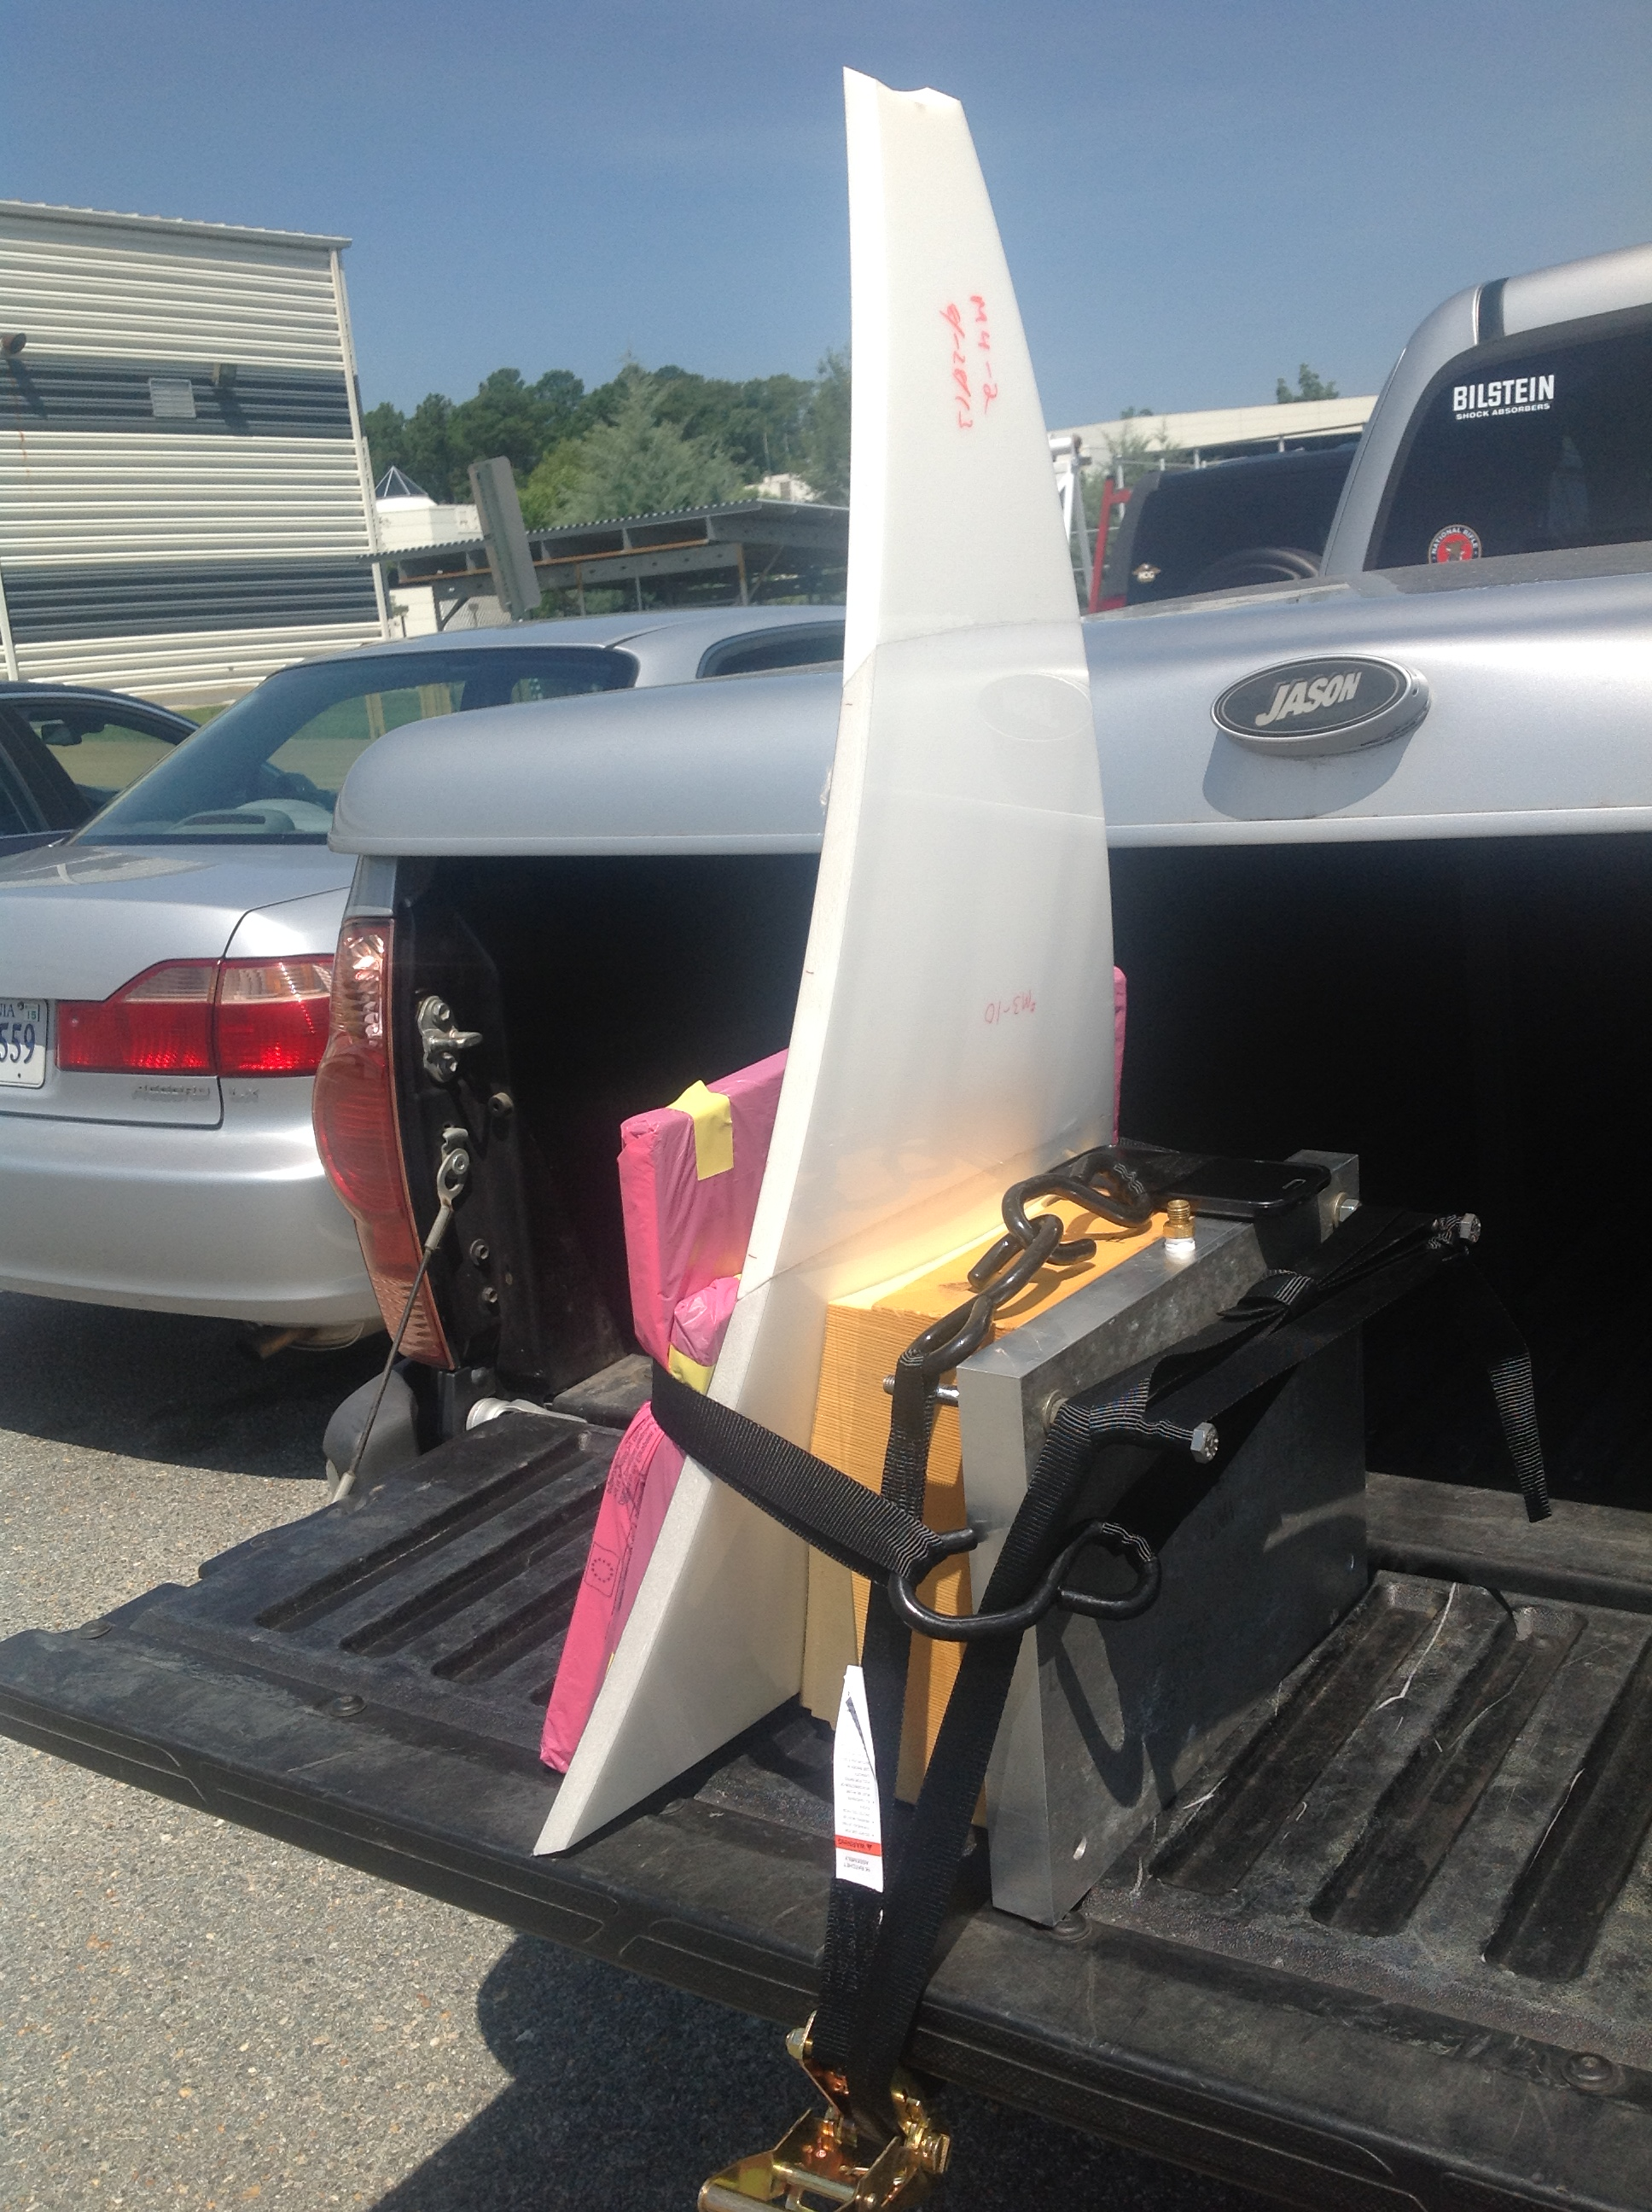
\includegraphics[trim={1.5cm 5cm 0 2cm }, clip, width=\linewidth]{images/Road_Test.JPG}
    \caption{Road tests of the spare mirror.}
    \label{fig:transportation_spare_mirror}
\end{figure}

%\begin{comment}
%  Road surface defects caused the mirror to accelerate, and this acceleration was measured at different speeds along
%  the route. The results obtained allowed us to determine the maximum speed with which the detector was supposed to
%  be transported, bearing in mind that it would be exposed to the external environment and, therefore, could be subject
%  to significant temperature changes if the transportation time was not limited in any way. 
%\end{comment}
  
The vessel had to be rigid, have negligible deformation while changing its orientation and, at the same time, allow
easy access to any internal component. There is one special requirement for the mirror support structure. The
Containment Vessel has only a limited rigidity and even small deformations could directly lead to a dangerous
deformation of the HTCC mirror if it was attached to the Containment Vessel directly in ordinary ways. Even if the
mirror remains whole and without any cracks, the light collection pattern could still be changed and decrease the
signal strength.

In general the vessel works as the support structure for all internal components and must be both light-tight and
gas-tight. Safety considerations require that we have both easy and safe access to the components inside. This is
absolutely necessary during maintenance and while running alignment checks. Special attention was paid to the cable
and fiber optics routing inside the volume. These items are very difficult to replace. The vessel is equipped with a
local gas distribution and a control panel. The control panel is for safe and continuous purging of the volume with
different dry gases (as needed) and used to keep the water vapor concentration level under tight control during
both operations and maintenance.

There was a need to have easy access to any of the 48 photomultiplier tubes (PMTs) to adjust their alignment and
for maintenance. The Containment Vessel has 24 service hatches wide enough to perform work on any channel. Each
channel consists of a PMT with high voltage divider, magnetic shield with compensation coil, and Winston Cone, which
are installed in the PMT mounting fixture together as one unit, see Fig.~\ref{fig:PMT_Mount}.

\begin{figure}[ht]
    \centering
    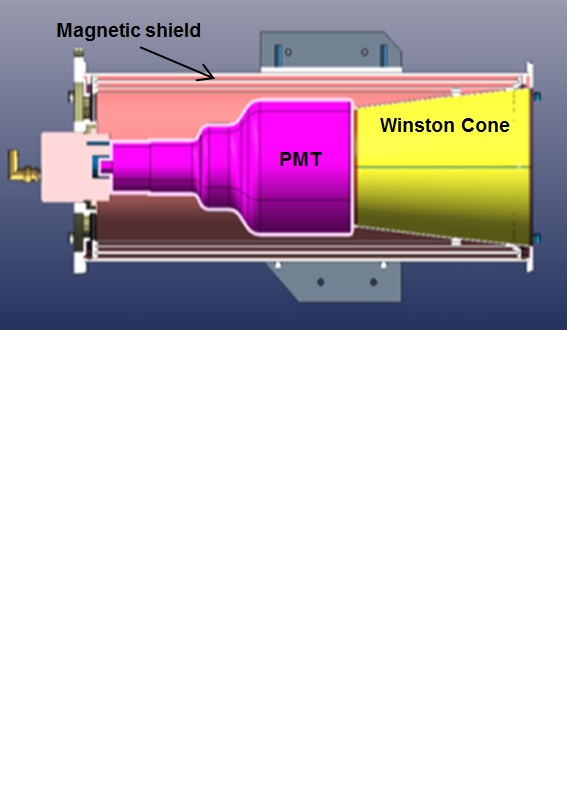
\includegraphics[width=1.0\linewidth,trim={0 12cm 0 0},clip]{images/PMT_Mount.jpg}
    \caption{PMT mounting unit with components.}
    \label{fig:PMT_Mount}
\end{figure}

Checks of the cabling and installed fiber optics used for calibration of the PMTs can also be done using the
service hatches. Service work can be performed on the detector while it is in its nominal working location. Any
access to the internal components of the detector requires replacement of the working gas with dry oxygen. For
safety a procedure of purging the HTCC volume has been established to allow access only when the concentration
of oxygen in the volume exceeds 19.5\%.

The combined HTCC mirror is supported and held in the Containment Vessel by 6 orthogonal links. These links
connect the supporting ring (attached to the mirror) to the Containment Vessel. It was critical that any deformation
of the Containment Vessel not be transmitted to the mirror. Each link has a ball-end swivel on each end. By using the
minimum number of links (6) to constrain all motion, the mirror could be aligned, but no forces above those due to
gravity on the mass of the mirror and its strong-back are ever placed on the mirror. The set of links are attached to
the Containment Vessel at 3 points that are spaced 120$^\circ$ around the perimeter of the ring. This scheme of
attachment was tested using a very light-weight 5-ft diameter flat mirror. The tests showed that the light collection
pattern stays unchanged within a sufficiently wide range of deformations of the frame that supported the mirror.
Therefore possible deformation of the Containment Vessel during installation and alignment do not affect the original
shape of the HTCC mirror. Figure~\ref{fig:HTCC_MIRR_INST_NEW} shows the HTCC mirror installed in the
Containment Vessel.

\begin{figure}[ht]
    \centering
    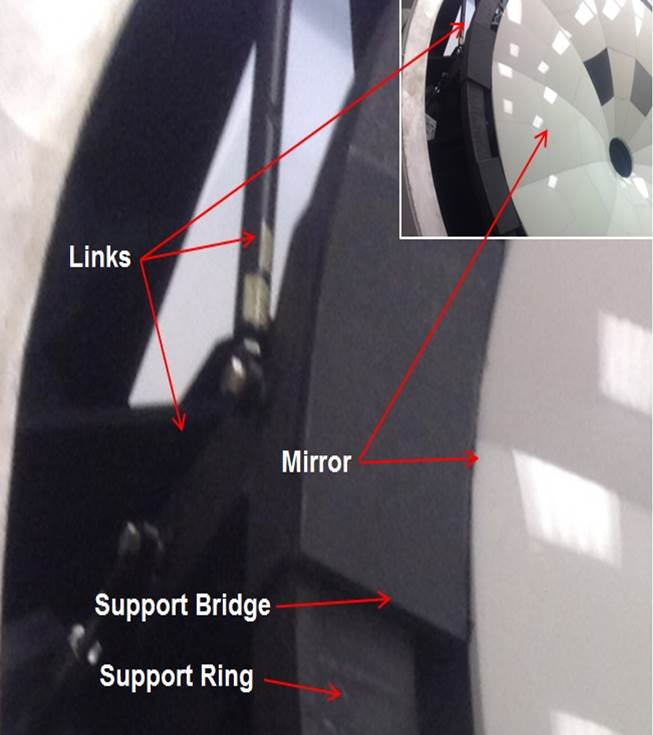
\includegraphics[width=1.0\linewidth,trim={0 0cm 0 0},clip]{images/HTCC_MIRR_INST_NEW.jpg}
    \caption{Combined mirror installed in the Containment Vessel. The set of links holding the mirror in position
      allow for fine adjustment with an accuracy of $\sim$0.01~in or better.}
    \label{fig:HTCC_MIRR_INST_NEW}
\end{figure}

The HTCC is susceptible to noticeable deformations due to the large overall dimensions of the detector. The light
and gas leak protection measures provided thus had to be reliable and require little maintenance. All of the inside
surfaces have been painted a flat black to reduce light reflectance, and all of the borders between adjacent parts
that form the outside shell of the detector have been sealed with a flexible black silicone gel on both the inside and
outside of the vessel. Sealing all the inside seams was necessary to allow the detector to always stay under a positive
differential pressure during variations in the atmospheric pressure. As a result of even small changes in the
differential pressure, the vessel would be deformed due to its large volume, i.e. the pressure is applied to a large
surface area. 

\subsection{Alignment of the Light Collection Components}

The HTCC contains light collection and light detection components: the mirror, Winston Light concentrators, and
photomultiplier tubes (PMTs). Even if the mirror is constructed and installed properly as designed, final checks of
the component alignment are needed. We have conducted comprehensive checks of the light collection optics on the
fully assembled detector. This work was done before the detector was moved to the experimental hall. For the
alignment checks we again used a low-power laser, gimbal mounted in the target position. To operate the laser we
used a set of standard high-precision devices to control the position and orientation of the laser. The opaque entry
window was replaced with a thin transparent film in order to keep the volume of the detector isolated as much as
possible. We opened one access hatch at the time for short periods of time to install templates on the face of the
accessible Winston cones and perform adjustments of the housing units each containing a 5-in PMT, Winston cone,
3-layer magnetic shield, and compensation coil. The alignment of all 48 PMT housing units was checked and adjusted
as needed.

Each mirror facet was illuminated with the laser at 5 points: the center of the facet and its four corners, and the
reflected light  pattern was photographed. For some of the channels we checked the light collection geometry at
normal relative humidity in the HTCC volume and at 0\% relative humidity. 

%\begin{comment}
%We allowed enough time for components to rich the required equilibrium.
%\end{comment}

Figure~\ref{fig:GEO_TEST_3_Normal} shows the pattern of the light reflection when mirror facet \#3 was
illuminated in the center. Circles of diameter 1~in, 3~in, and 5~in concentric to the PMT are shown. The result was
obtained at normal relative humidity. Results obtained at RH=0\% for the same channel show small but acceptable
differences (see Fig.~\ref{fig:GEO_TEST_3_Zero}). Similar geometry test results were obtained for channel
\#4 covering polar angles in range of $5^\circ$ to $12.5^\circ$. They are shown in the
Figs.~\ref{fig:GEO_TEST_4_Normal} and ~\ref{fig:GEO_TEST_4_Zero} obtained at different relative humidities.

Considering the light collection patterns obtained when the mirror facets were illuminated in the corners we made
the necessary adjustments in the alignment of the PMT mounting units. No adjustments were needed for the HTCC
mirror. Figure~\ref{fig:Ch_5_1_3_Before_NEW} shows the test results for mirror facet \#3 from Sector 5,
half-sector 1 obtained before adjustments in alignment were done. Figure~\ref{fig:Ch_5_1_3_After_NEW} shows
the changes in the light collection pattern after the alignment adjustments. The image has been shifted toward the
center. Figure~\ref{fig:GEO_TEST_5_1_3_Center} shows a photograph taken when the mirror was illuminated in
the center. The five circles concentric to the PMT shown in the picture have diameters from 1 to 6~in. 

\begin{figure}[ht]
    \centering
    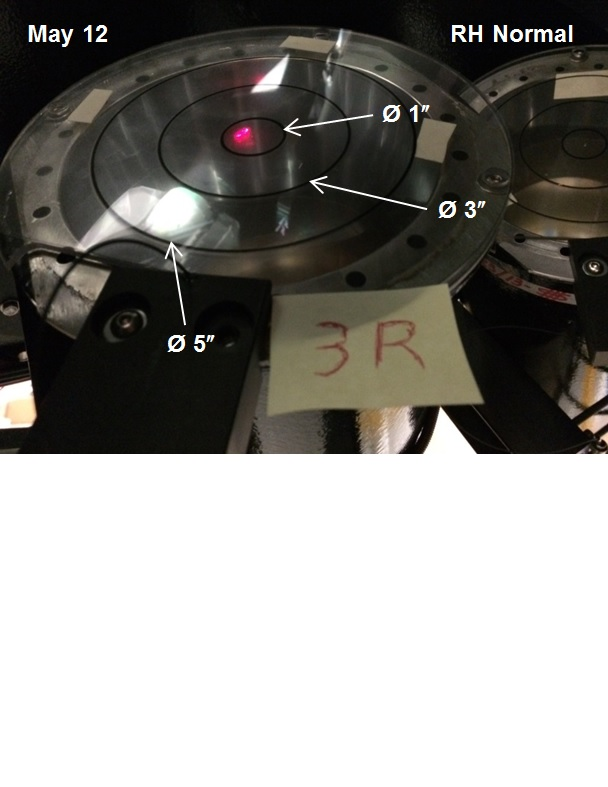
\includegraphics[width=1.0\linewidth,trim={0 8.5cm 0 0},clip]{images/GEO_TEST_3_Normal.jpg}
    \caption{Geometry test result for channel \#3 covering polar angles from $12.5^\circ$ to $20^\circ$ at
      nominal relative humidity. The corresponding mirror facet was illuminated in the center.}
    \label{fig:GEO_TEST_3_Normal}
\end{figure}

\begin{figure}[ht]
    \centering
    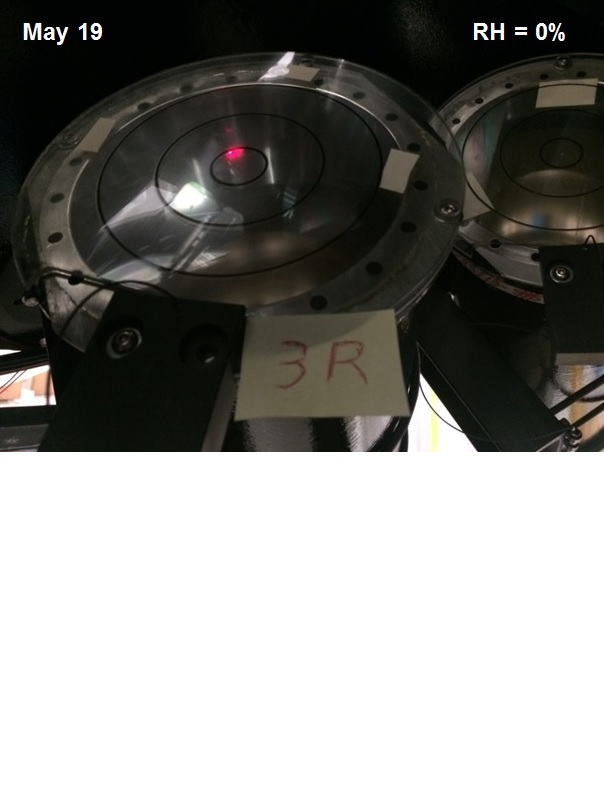
\includegraphics[width=1.0\linewidth,trim={0 8.5cm 0 0},clip]{images/GEO_TEST_3_Zero.jpg}
    \caption{Geometry test result for channel \#3 covering polar angles from $12.5^\circ$ to $20^\circ$
      at RH=0\%. The corresponding mirror facet was illuminated in the center.}
    \label{fig:GEO_TEST_3_Zero}
\end{figure}
        
\begin{figure}[ht]
    \centering
    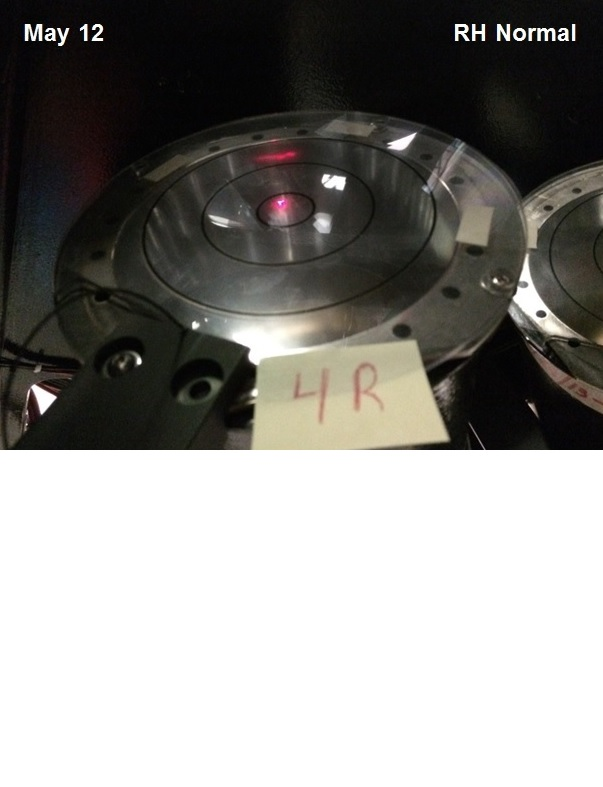
\includegraphics[width=1.0\linewidth,trim={0 8.5cm 0 0},clip]{images/GEO_TEST_4_Normal.jpg}
    \caption{Geometry test result for channel \#4 covering polar angles from $5^\circ$ to $12.5^\circ$ at
      nominal relative humidity. The corresponding mirror facet was illuminated in the center.}
    \label{fig:GEO_TEST_4_Normal}
\end{figure}

\begin{figure}[ht]
    \centering
    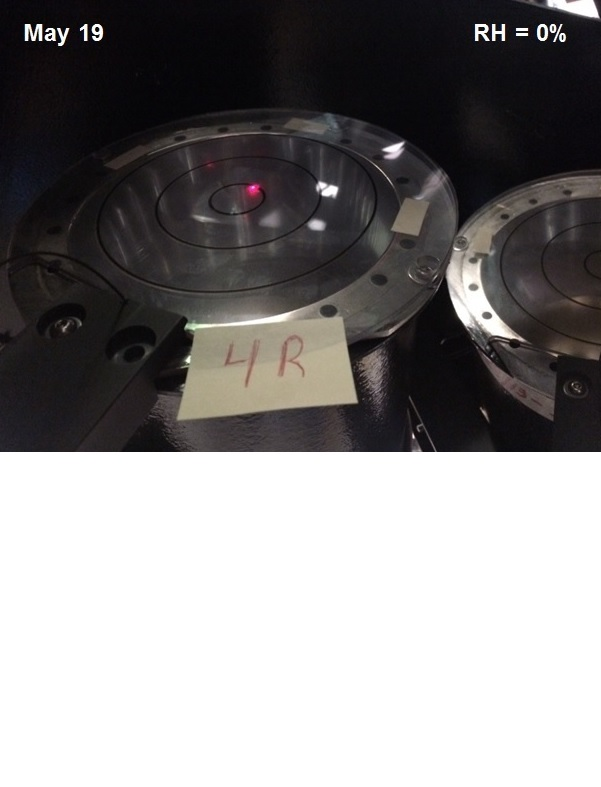
\includegraphics[width=1.0\linewidth,trim={0 8.5cm 0 0},clip]{images/GEO_TEST_4_Zero.jpg}
    \caption{Geometry test result for channel \#4 covering polar angles from $5^\circ$ to $12.5^\circ$ at
      RH=0\%. The corresponding mirror facet was illuminated in the center.}
    \label{fig:GEO_TEST_4_Zero}
\end{figure}

\begin{figure}[ht]
    \centering
    \includegraphics[width=1.0\linewidth,trim={0 0cm 0 0},clip]{images/Ch_5_1_3_Before_NEW.jpg}
    \caption{Geometry test result for the sector 5, half-sector 1, mirror \#3 covering polar angles in range of
      $12.5^\circ$ to $20^\circ$ obtained before adjustment when mirror \#3 was illuminated in the center (blue),
      and its corners (purple). The black circles are 1~in to 6~in in diameter. The circle (red) is of radius 0.45~in,
      and is equal to the RMS of the fitted center of gravity of the light collection pattern.}
    \label{fig:Ch_5_1_3_Before_NEW}
\end{figure}

\begin{figure}[ht]
    \centering
    \includegraphics[width=1.0\linewidth,trim={0 0cm 0 0},clip]{images/Ch_5_1_3_After_NEW.jpg}
    \caption{Geometry test result for the sector 5, half-sector 1, mirror \#3 covering polar angles in range of
      $12.5^\circ$ to $20^\circ$ obtained after adjustment when mirror \#3 was illuminated in the center (blue) and
      its corners (purple). The black circles are 1~in to 6~in in diameter. The circle (red) is of radius 0.51~in, and is
      equal to the RMS of fitted center of gravity  of the light collection pattern.}
    \label{fig:Ch_5_1_3_After_NEW}
\end{figure}

\begin{figure}[ht]
    \centering
    \includegraphics[width=1.0\linewidth,trim={0 0cm 0 0},clip]{images/GEO_TEST_5_1_3_Center.jpg}
    \caption{Geometry test result for the sector 5, half-sector 1, mirror \#3 covering polar angles in range of
      $12.5^\circ$ to $20^\circ$ obtained after adjustment when mirror \#3 was illuminated in the center.}
    \label{fig:GEO_TEST_5_1_3_Center}
\end{figure}

Figure~\ref{fig:subfig} shows the final light collection patterns obtained for all mirrors for half-sectors 1 and
2 from sector~5. One can clearly see that the light collection is more focused for the small mirrors than for the
large ones. This effect is caused by the difference in the rigidity between the combined mirror itself and the
supporting ring attached to it, as well as the different sensitivities to the changes in relative humidity of the
environment.
 
%\begin{comment}
%  As we have observed the fully assembled combined mirror wood stay similar to itself with relatively small changes in
%  its overall dimensions  if relative humidity is changing from normal to low. The support ring is insensitive to such
%  humidity changes. This two components are glued together with glue which is relatively elastic as compared with
%  epoxy. But still changes in diameter of the mirror due to humidity generates a certain force stretching the relatively
%  elastic glue joint between ring and the mirror. In other words the mirror is being radially stretched. 
%\end{comment}

Since the mirror has a funnel shape, see Fig.~\ref{fig:Colored_Mirror}, the nose of the funnel gets stretched
less than outer portion of the mirror. The outer portion of the mirror consists of mirror facets \#1 and \#2, the
largest mirror facets. Even though the widths of facets \#1 and \#2 measured in the radial direction are close to
each other, the effect of humidity changes for the outermost facet \#1 is larger than for facet \#2 due to the
funnel shape of the combined mirror.

\begin{figure*}
\begin{subfigure}[b]{0.49\textwidth}
    \includegraphics[width=1.0\textwidth]{images/GEO_TEST_Sect5_M_1_M_2.jpg}
    \caption{} \label{fig:subfig1_a}
\end{subfigure}
\hspace*{\fill} % separation between the subfigures
\begin{subfigure}[b]{0.5\textwidth}
    \includegraphics[width=1.0\linewidth]{images/GEO_TEST_Sect5_M_3_M_4.jpg}
    \caption{} \label{fig:subfig1_b}
\end{subfigure}
\caption{Light collection test result for both half-sectors of Sector 5. (a) - Mirrors \#1 and \#2 cover polar
  angles in range of $20^\circ$ to $35^\circ$  within an azimuthal interval of $60^\circ$. (b) - Mirrors \#3 and
  \#4 cover polar angles in range of $5^\circ$ to $20^\circ$  within an azimuthal interval of $60^\circ$. The data
  are shown after adjustment of the light-collection optics. The mirrors were illuminated in the center and the
  corners.} 
\label{fig:subfig}
\end{figure*}

\begin{figure}[ht]
    \centering
    \includegraphics[width=1.0\linewidth,trim={0 0cm 0 0},clip]{images/Colored_Mirror.jpg}
    \caption{The combined HTCC mirror is funnel-shaped.}
    \label{fig:Colored_Mirror}
\end{figure}

\subsection{Gas Composition Control}

The fully assembled detector was tested for gas and light leaks. Gas tightness was checked by filling the volume
with a mixture of dry air and a small amount of non-flammable gas at positive differential pressure. Freon gas leak
sniffers were used. As expected, most of the leaks were found around the entry and exit windows because both
windows were sealed only from the outside as they were the last two components attached to the Containment
Vessel. Light tightness was checked by monitoring the counting rates of the photomultiplier tubes while illuminating
the sealed seams of the vessel with an external light source. The rates were close to the dark counting rates whether
the lights in the hall were turned on or off. The gas tightness was controlled by fixing the leaks found and then by
measuring the humidity inside the detector while it was continuously purged with dry nitrogen. At flow rates of
10 - 15~l/min, a humidity level not higher than $\sim$100~ppm was measured in a span of 2-3~days of continuous
purging. These results can be used as a good indication of a low level of water vapor and oxygen content. Note that
the diffusion of water vapor and oxygen through the windows is defined by the Tedlar films, which have the lowest
diffusion coefficients. For Tedlar the diffusion of oxygen is lower than the diffusion of water vapor. The presence of
water vapor and oxygen in the working volume is unavoidable but should be kept at the lowest possible level because
water vapor and CO${_2}$ gas produce carbonic acid that may be harmful to the mirror working surface. As far as
oxygen content is concerned, it also needs to be kept at the lowest possible level. During operations with beam a
certain amount of ozone can be generated due to radiation. Both oxygen and ozone absorb the ultraviolet component
of Cherenkov light in the HTCC generated by scattered electrons. Consequently the signal strength becomes lower,
which directly leads to a reduced rejection of charged pions.

%\begin{comment}
%  Almost one year has passed since CLAS12 operations with beam started, and no degradation of signal strength has
%  been observed, which means that all controlled parameters are stable. But still actual composition and possible
%  changes of the radiator gas is unknown. We plan installation of the residual gas analyzer to  continuously monitor the
%  concentration of oxygen, ozone and helium gases. Helium is especially harmful for the PMTs with quartz windows.
%  Quartz entry windows are freely penetrated by helium gas, and the introduction of helium would ruin the vacuum in
%  the PMT. The ozone and helium are generated during running experiments. The ozone is due to radiation, and the
%  presence of helium is due to the operations of the superconducting Torus magnet and Central Solenoid magnet in
%  the hall. Since more than 50\% of the containment vessel surface are covered with plastics the only tool to better
%  control gas composition would be usage of the reasonably high rate of purging.
%\end{comment}

Another reason to keep tight control on humidity is related to the sensitivity (to some extent) of the mirror shape
to humidity. The mirror must be used at the lowest humidity level, but the entire manufacturing process of the
mirror facets was done at normal room conditions. Once the mirror had been installed, the HTCC volume was sealed
and purged with dry gas (N${_2}$, CO${_2}$, or dry air). Altering the humidity from almost zero to normal
atmosphere conditions may lead to component fatigue and cause structural deformation. During maintenance the
volume is partially exposed to the outside environment, which increases humidity. In any case, all maintenance
activities are stopped once the relative humidity inside the volume reaches 2-3\%. This is controlled at the exhaust
of the detector. Maintenance is resumed only after the operational humidity level is restored. The detector is
equipped with a local gas control panel. The parameters that can be read directly are limited to the pressure at the
input of the volume and the differential pressure. The HTCC is continuously monitored online by a system that
monitors the following parameters:

\begin{itemize}
    \item Type of gas;
    \item Gas flow rate;
    \item Differential pressure;
    \item Humidity;
    \item Amount of gas already consumed.
\end{itemize}

The online control system allows the detector to be safely operated within predefined intervals of parameter
variations. This system generates warnings and alarms that require either remote or in situ response. In the case of
a power outage in the hall, the mass flow controller turns off and purging is stopped. It takes several hours for the
humidity to rise up to 2-3\% due to direct leaks and diffusion of the ambient humid air inside the working volume.
This provides enough time for operation to switch the gas to a manual bypass rota-meter, which is normally closed.
The local gas panel includes three specialized filters that prevent dust, water vapor, and oil vapor from entering
the volume.

%\begin{comment}
%  There was a need to have easy access to any of the 48 PMTs to adjust their alignment and for maintenance. The
%  Containment Vessel has 24 service hatches wide enough to perform work on any channel. Each channel consists of
%  a PMT with high voltage divider, magnetic shield with compensation coil, and Winston Cone, which are installed in
%  the PMT mounting fixture together as one unit, see Fig.~\ref{fig:PMT_Mount}.
%
%\begin{figure}[ht]
%    \centering
%    \includegraphics[width=1.0\linewidth,trim={0 12cm 0 0},clip]{images/PMT_Mount.jpg}
%    \caption{PMT mounting unit with components.}
%    \label{fig:PMT_Mount}
%\end{figure}
%
%Checks of cabling and installed fiber optics used for calibration of the PMTs also can be done using service hatches.
%Service work can be performed on the detector while it is in nominal working location. Any access to the internal
%components of the detector require replacement of the working gas with dry oxygen. For safety the corresponding
%procedure of purging the HTCC volume has been established to allow access only in when the concentration of oxygen
%in the volume exceeds 19.5\%.
%\end{comment}
